\documentclass[11pt]{article}
\usepackage[T1]{fontenc}
\usepackage{lmodern}
\usepackage{parskip}
\usepackage[colorlinks=true,urlcolor=blue,linkcolor=black,citecolor=black]{hyperref}
\usepackage{graphicx}
\usepackage{amsmath}
\usepackage[utf8]{inputenc}
\usepackage[spanish]{babel}
\usepackage{fancyhdr}
\usepackage{csquotes}
\usepackage{lastpage}
\usepackage{array}
\usepackage{listings}
\usepackage{color}
\definecolor{dkgreen}{rgb}{0,0.6,0}
\definecolor{gray}{rgb}{0.5,0.5,0.5}
\definecolor{mauve}{rgb}{0.58,0,0.82}
\usepackage[affil-it]{authblk}
\usepackage[activate={true,nocompatibility},final,tracking=true,kerning=true,spacing=true,factor=1100,stretch=10,shrink=10]{microtype}
\usepackage[hmargin=2cm,top=4cm,headheight=65pt,footskip=65pt]{geometry}
\usepackage{hyperref}
\usepackage{graphicx}
\usepackage{float}
\usepackage{tabularx}
\graphicspath{ {./screenshots/} }

% Documento
\begin{document}

\begin{titlepage}
 \begin{center}
        \vspace*{1cm}
            
        \Huge
        \textbf{Prácticas de Laboratorio}
            
        \vspace{0.5cm}
        \LARGE
        Informática Forense y Auditoría
            
        \vspace{1.5cm}
            
        \textbf{Hugo Fonseca Díaz}\\
        UO258318\\
        \href{mailto:uo258318@uniovi.es}{uo258318@uniovi.es}
            
        \vfill
            
        Convocatoria Junio-Julio 2021.
            
        \vspace{0.8cm}
            
        
\includegraphics[width=0.3\textwidth]{other/uniovi_logo.jpg}
            
        \Large
        Escuela de Ingeniería Informática\\
        Universidad de Oviedo\\
        España\\
        28 de junio de 2021
            
    \end{center}
\end{titlepage}

\newpage

\tableofcontents

\newpage

% Introducción
\section{Introducción}
Los ejercicios de este documento se han realizado en una máquina cuyas características se muestran en la siguiente captura.

\begin{figure}[H]
  \caption{Sistema del alumno Hugo Fonseca Díaz.}
  \centering
    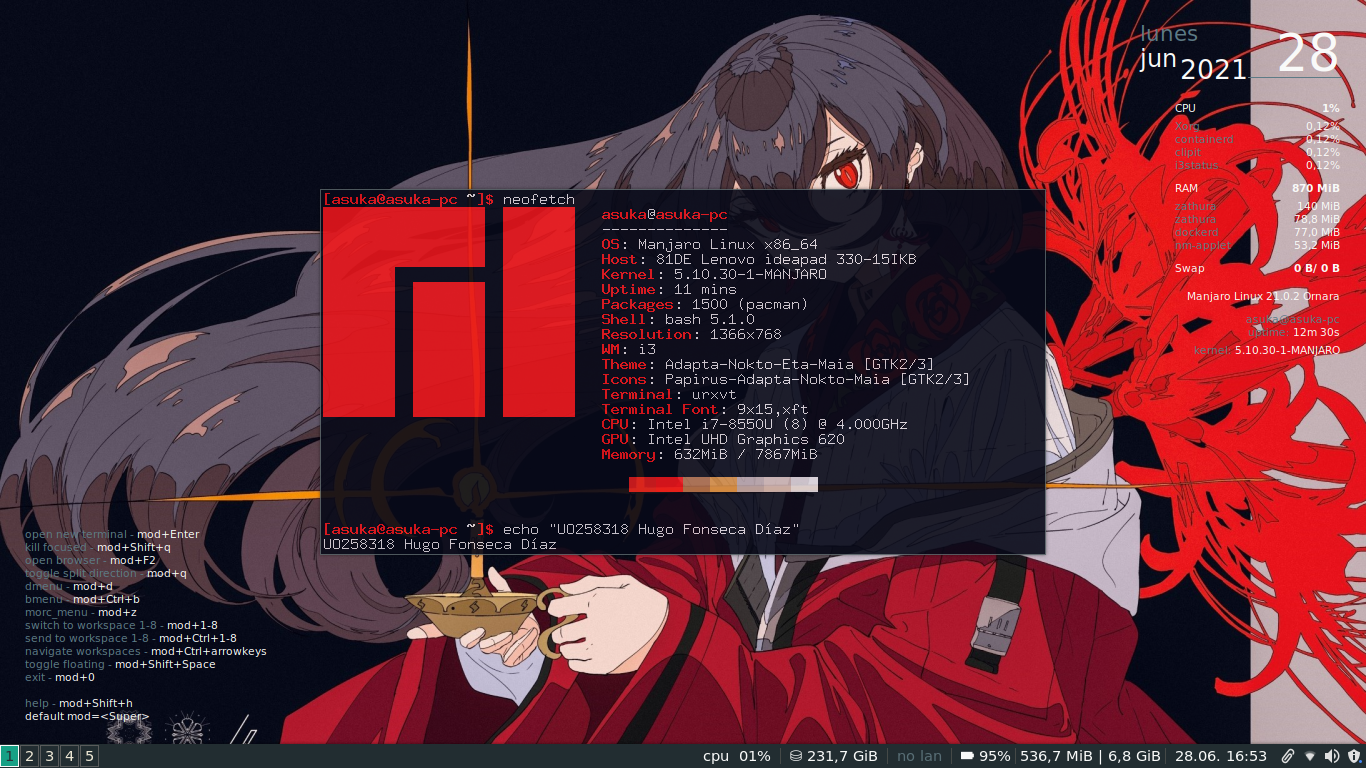
\includegraphics[scale=0.4, trim={0 1cm 0 0}, clip]{other/sistema_hugo.png}
\end{figure}

Las máquinas virtuales utilizadas pueden verse en la siguiente imagen.

\begin{figure}[H]
  \caption{Máquinas virtuales.}
  \centering
    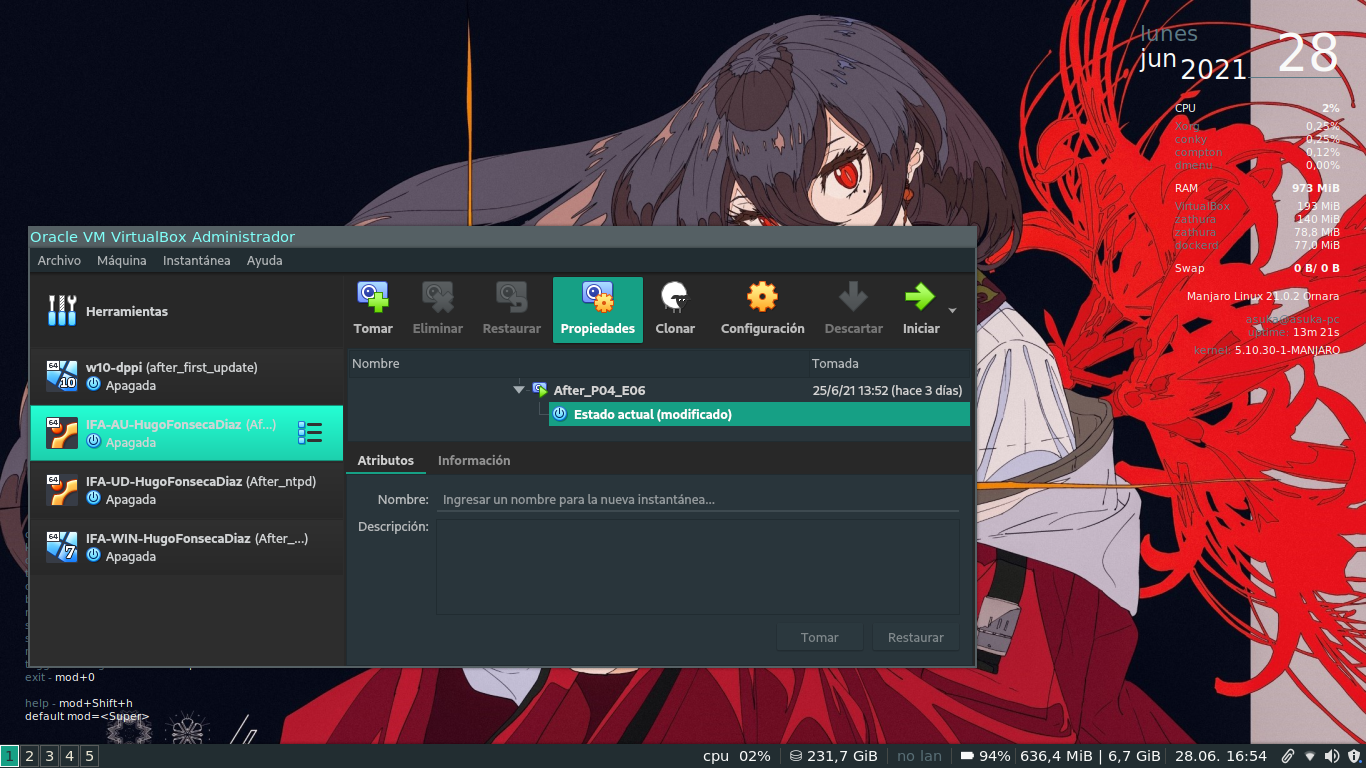
\includegraphics[scale=0.4, trim={0 1cm 0 0}, clip]{other/maquinas_virtuales_hugo.png}
\end{figure}

% Práctica 02
\section{Práctica 02}

\subsection{Ejercicio 27}

\begin{figure}[H]
    \caption{Ejercicio 27: Enunciado.}
  \centering
  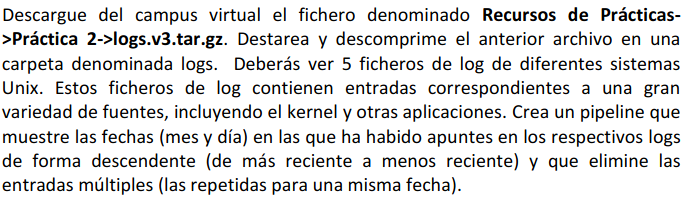
\includegraphics[scale=0.7]{other/enunciado_p02_e27.png}
\end{figure}

Se descomprime el archivo con el comando \verb|tar| y las flags \textit{xvzf}, siendo \textit{x} una indicación de que se quiere extraer los contenidos del archivo comprimido, \textit{v} para que lo haga de manera verbosa, \textit{z} para indicarle al comando que el archivo es un zip y \textit{f} para pasarle el fichero que se desea extraer al comando.

\begin{figure}[H]
    \caption{Ejercicio 27: \textit{tar -xvzf}.}
  \centering
  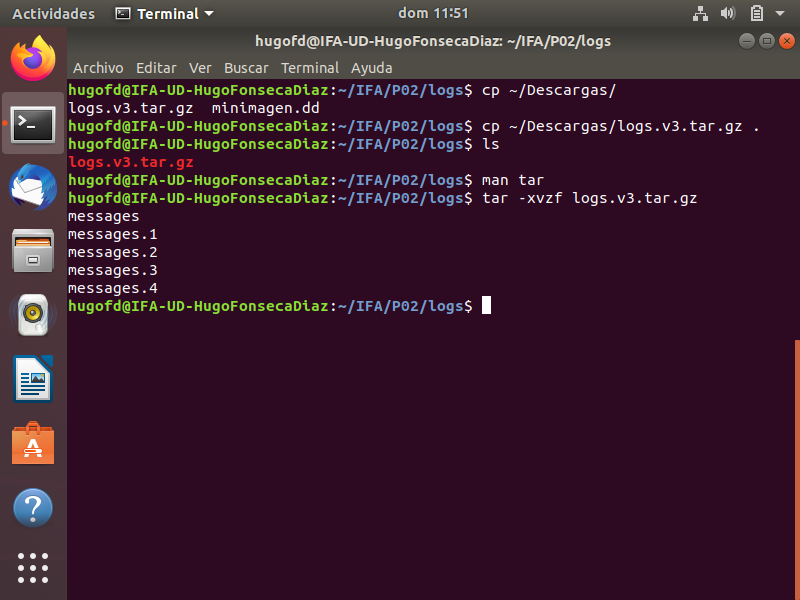
\includegraphics[scale=0.7, trim={0 7cm 0 0}, clip]{p02/e27-1.png}
\end{figure}

Una vez descomprimidos los ficheros de texto, se procede a utilizar tres nuevas herramientas. Se usa \verb|tac| para concatenar ficheros de forma inversa (es el comando \verb|cat| invertido), el lenguaje de programación AWK para procesar texto y el comando \verb|uniq| para omitir líneas repetidas.

\begin{figure}[H]
    \caption{Ejercicio 27: \textit{tac, AWK y uniq}.}
  \centering
  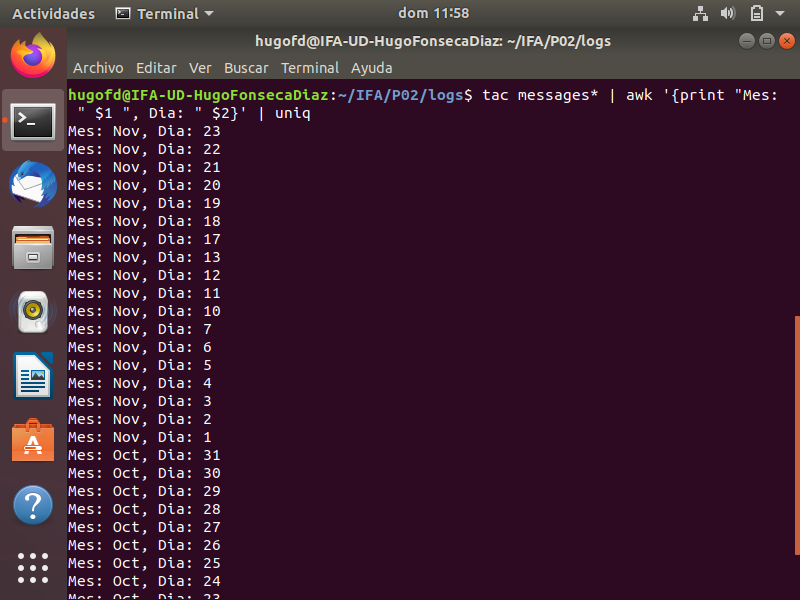
\includegraphics[scale=0.7]{p02/e27-2.png}
\end{figure}

\subsection{Ejercicio 31}

\begin{figure}[H]
    \caption{Ejercicio 31: Enunciado (I).}
  \centering
  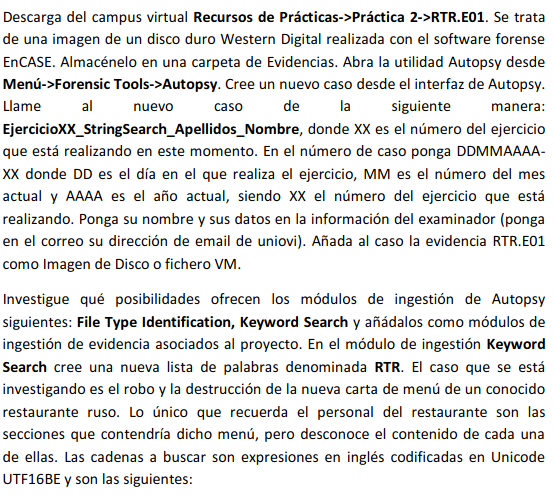
\includegraphics[scale=0.7]{other/enunciado_p02_e31-1.png}
\end{figure}

\begin{figure}[H]
    \caption{Ejercicio 31: Enunciado (II).}
  \centering
  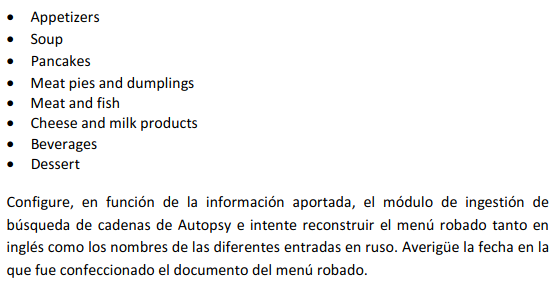
\includegraphics[scale=0.7]{other/enunciado_p02_e31-2.png}
\end{figure}

Se crea el caso en Autopsy con los datos solicitados.

\begin{figure}[H]
    \caption{Ejercicio 31: Creación del caso}
  \centering
  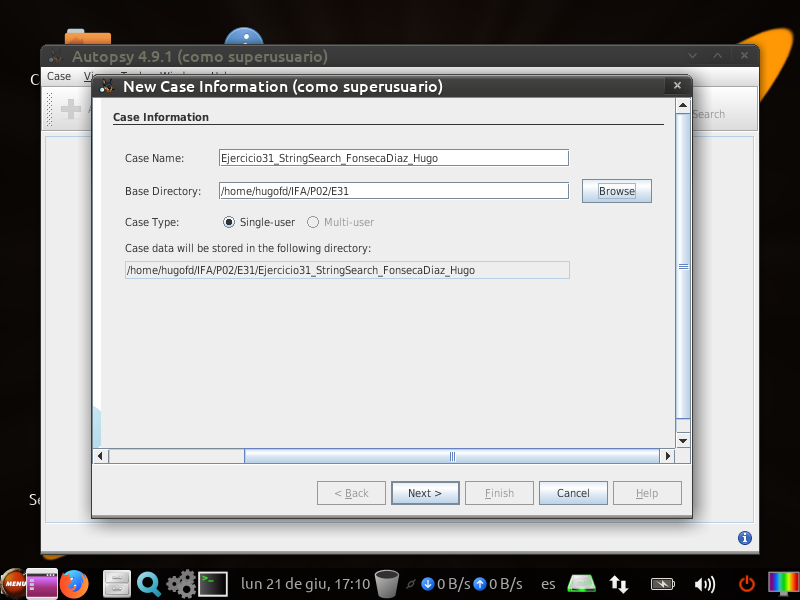
\includegraphics[scale=0.7]{p02/e31-1.png}
\end{figure}

\begin{figure}[H]
    \caption{Ejercicio 31: Selección de la imagen a analizar}
  \centering
  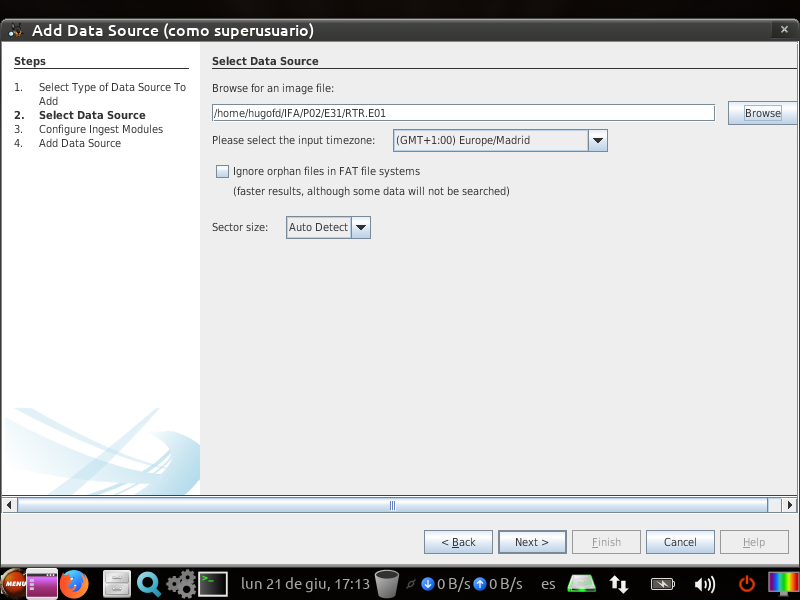
\includegraphics[scale=0.7]{p02/e31-2.png}
\end{figure}

Se seleccionan los módulos y se configura el módulo de búsqueda de palabras clave.

\begin{figure}[H]
    \caption{Ejercicio 31: Palabras clave}
  \centering
  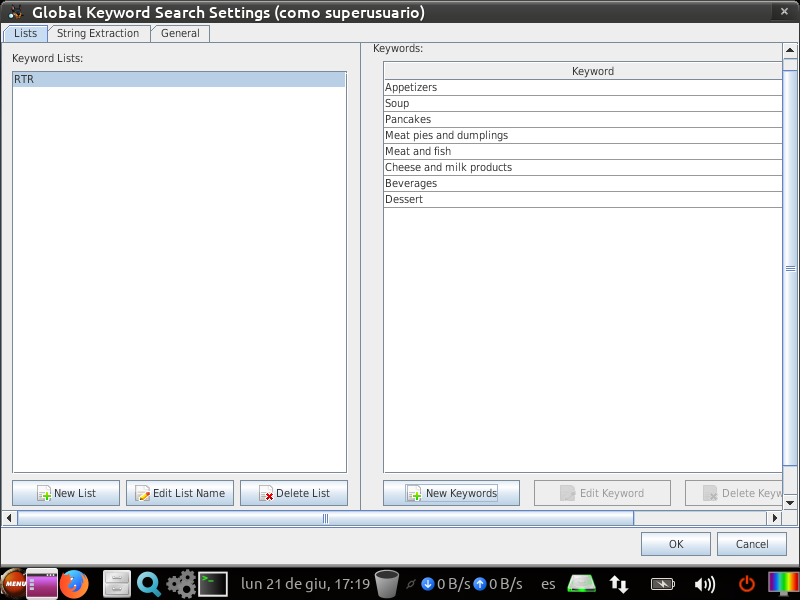
\includegraphics[scale=0.7]{p02/e31-3.png}
\end{figure}

\begin{figure}[H]
    \caption{Ejercicio 31: Módulos seleccionados}
  \centering
  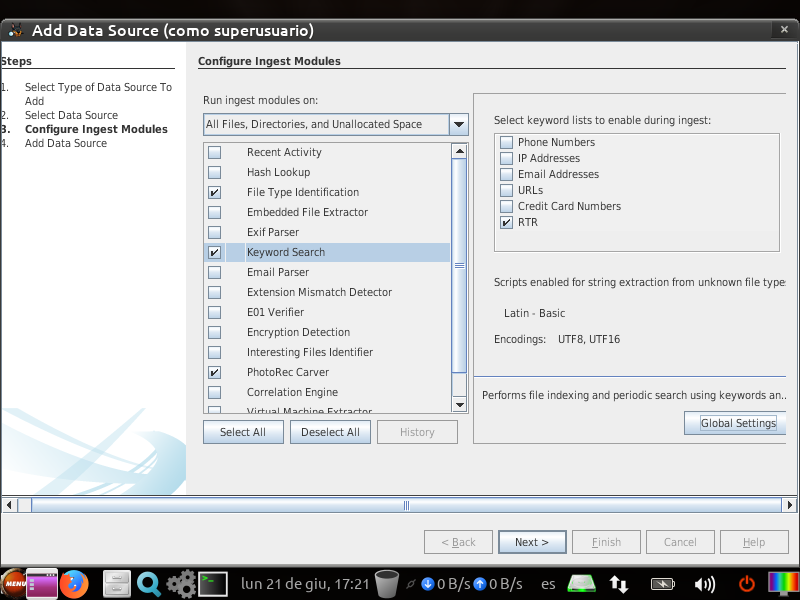
\includegraphics[scale=0.7]{p02/e31-4.png}
\end{figure}

\begin{figure}[H]
    \caption{Ejercicio 31: Configuración de los lenguajes de la búsqueda}
  \centering
  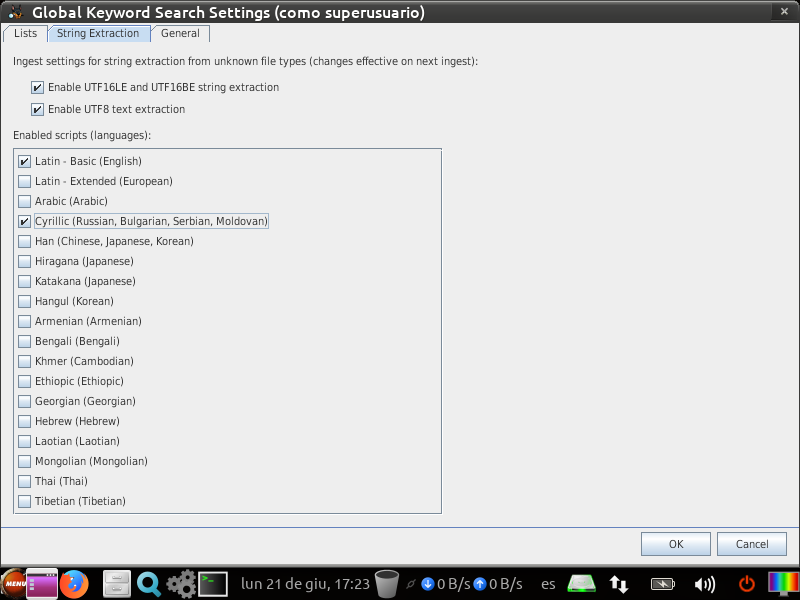
\includegraphics[scale=0.7]{p02/e31-5.png}
\end{figure}

Una vez finalizado el análisis, se pueden observar los ficheros encontrados.

\begin{figure}[H]
    \caption{Ejercicio 31: Resultados del análisis}
  \centering
  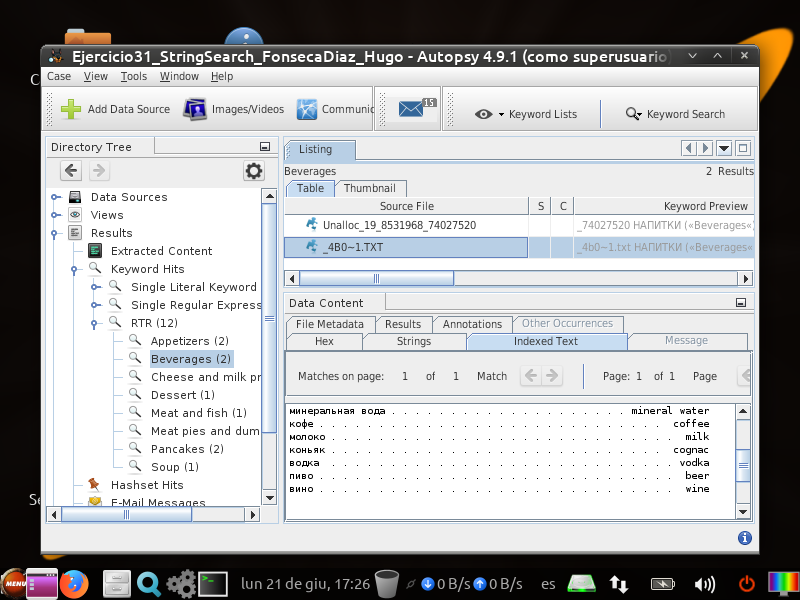
\includegraphics[scale=0.7]{p02/e31-6.png}
\end{figure}

Se reconstruye el menú del restaurante, creado inicialmente el 3 de noviembre de 2004.

\begin{figure}[H]
    \caption{Ejercicio 31: Menú reconstruido}
  \centering
  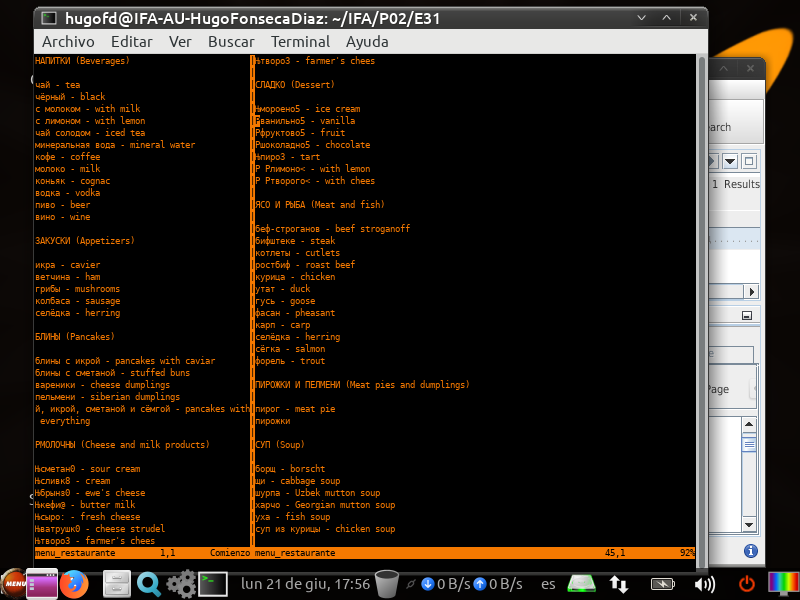
\includegraphics[scale=0.7]{p02/e31-7.png}
\end{figure}



% Práctica 03
\section{Práctica 03}

\subsection{Ejercicio 8}

\begin{figure}[H]
    \caption{Ejercicio 8: Enunciado.}
  \centering
  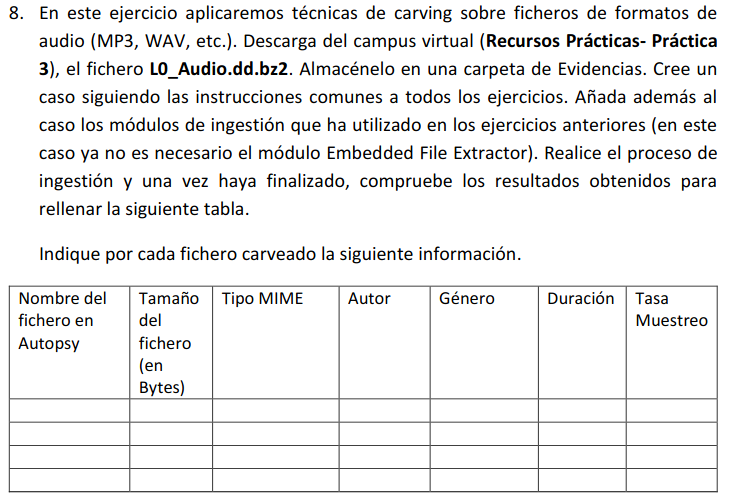
\includegraphics[scale=0.7]{other/enunciado_p03_e8.png}
\end{figure}

Se crea el caso en Autopsy con los datos solicitados.

\begin{figure}[H]
    \caption{Ejercicio 8: Creación del caso}
    \centering
    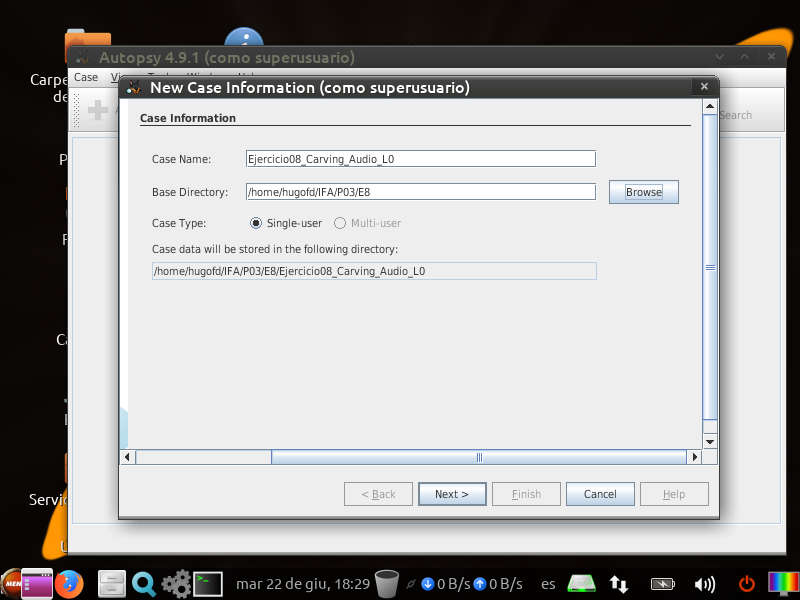
\includegraphics[scale=0.7]{p03/e8-1.png}
\end{figure}

\begin{figure}[H]
    \caption{Ejercicio 8: Detalles del examinador}
    \centering
    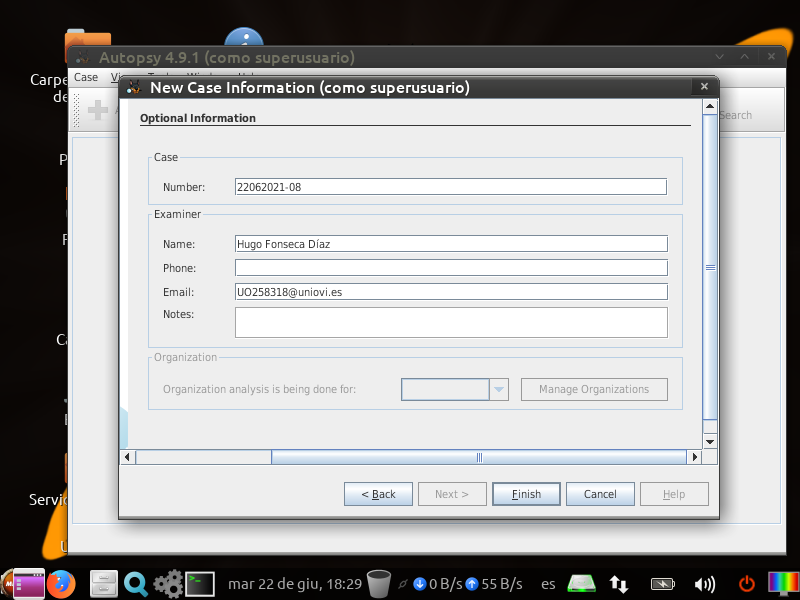
\includegraphics[scale=0.7]{p03/e8-2.png}
\end{figure}

Añadimos la imagen a analizar.

\begin{figure}[H]
    \caption{Ejercicio 8: Selección de la imagen}
    \centering
    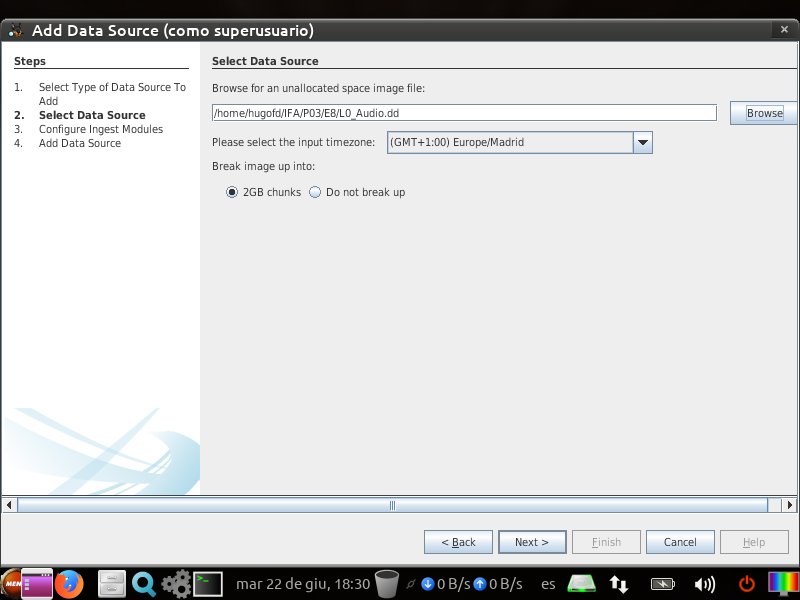
\includegraphics[scale=0.7]{p03/e8-3.png}
\end{figure}

Se seleccionan los módulos de identificación de tipos de fichero, parseador de Exif y \textit{PhotoRec Carver}.

\begin{figure}[H]
    \caption{Ejercicio 8: Selección de módulos}
    \centering
    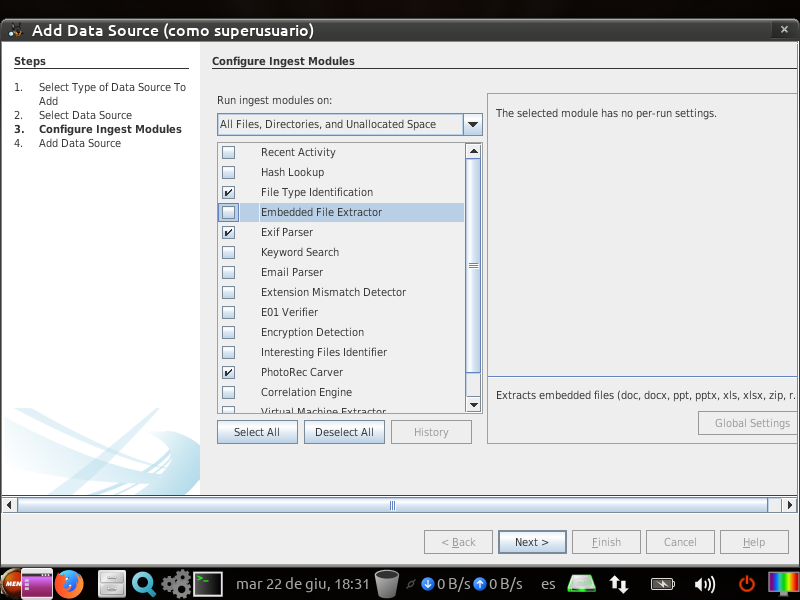
\includegraphics[scale=0.7]{p03/e8-4.png}
\end{figure}

Para rellenar la tabla se usarán los datos obtenidos al ejecutar el análisis de Autopsy y mediante el uso de la herramienta \textit{MediaInfo}.

\begin{figure}[H]
    \caption{Ejercicio 8: Resultados del análisis}
    \centering
    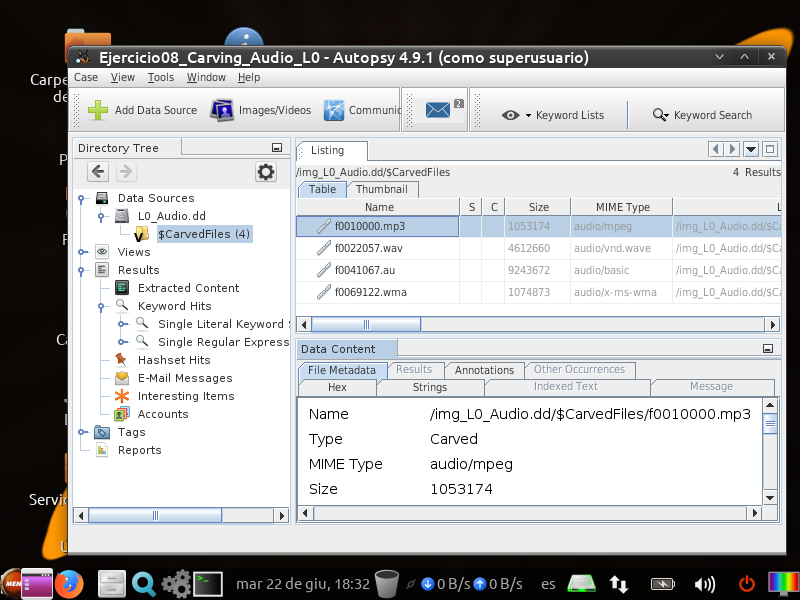
\includegraphics[scale=0.7]{p03/e8-5.png}
\end{figure}

\begin{figure}[H]
    \caption{Ejercicio 8: Herramienta \textit{MediaInfo}}
    \centering
    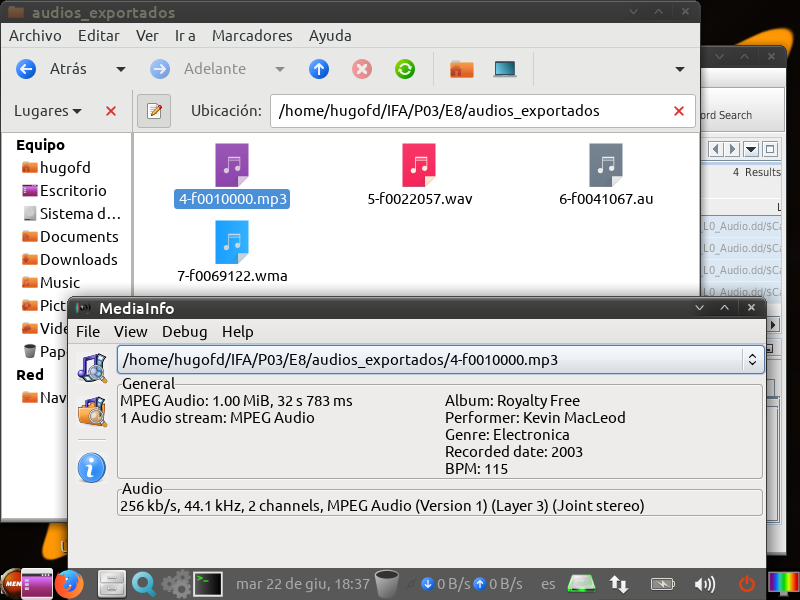
\includegraphics[scale=0.7]{p03/e8-6.png}
\end{figure}

\begin{table}[H]
    \centering
    \begin{tabular}{|p{2.5cm}|p{2cm}|c|p{1.5cm}|c|c|c|}
        \hline
        Nombre del fichero en Autopsy & Tamaño del fichero (en Bytes) & Tipo MIME & Autor & Género & Duración & Tasa de Muestreo \\
        \hline\hline
        f0010000.mp3 & 1053174 & audio/mpeg & Kevin McLeod & Electronica & 32s 783ms & 44.1kHz \\
        \hline
        f0022057.wav & 4612660 & audio/vnd.wave & - & - & 26s 148ms & 44.1kHz \\
        \hline
        f0041067.au & 9243672 & audio/basic & - & - & 3min 29s & 44.1kHz \\
        \hline
        f0069122.wma & 1074873 & audio/x-ms-wma & - & (80) & 1min 5s & 44.1kHz \\
        \hline
    \end{tabular}
\end{table}

\subsection{Ejercicio 13}

\begin{figure}[H]
    \caption{Ejercicio 13: Enunciado (I).}
  \centering
  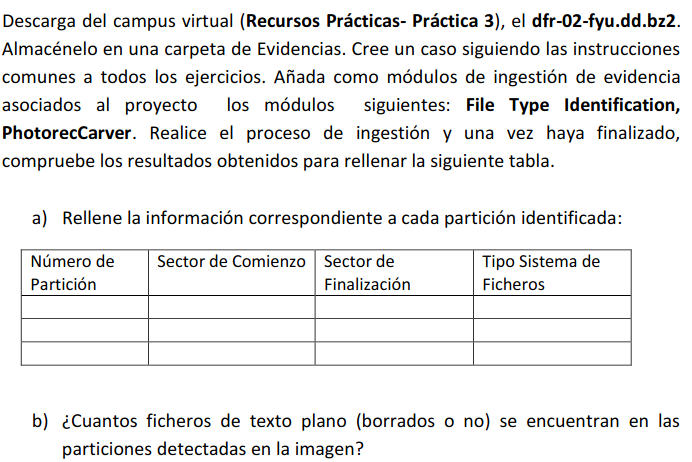
\includegraphics[scale=0.7]{other/enunciado_p03_e13-1.png}
\end{figure}

\begin{figure}[H]
    \caption{Ejercicio 13: Enunciado (II).}
  \centering
  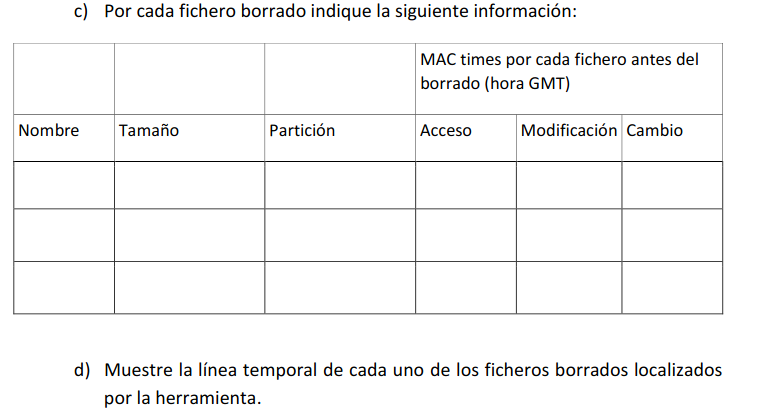
\includegraphics[scale=0.7]{other/enunciado_p03_e13-2.png}
\end{figure}

Se crea el caso en Autopsy con los datos solicitados.

\begin{figure}[H]
    \caption{Ejercicio 13: Creación del caso}
    \centering
    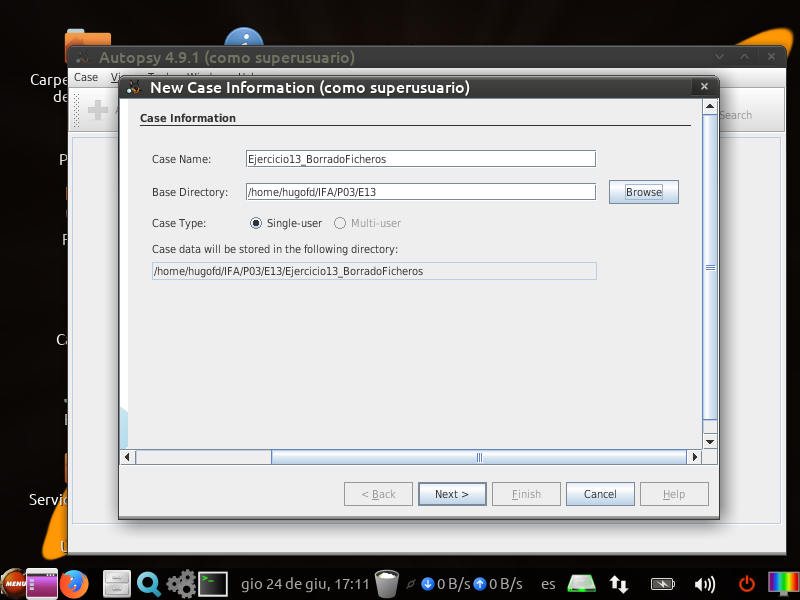
\includegraphics[scale=0.7]{p03/e13-1.png}
\end{figure}

\begin{figure}[H]
    \caption{Ejercicio 13: Detalles del examinador}
    \centering
    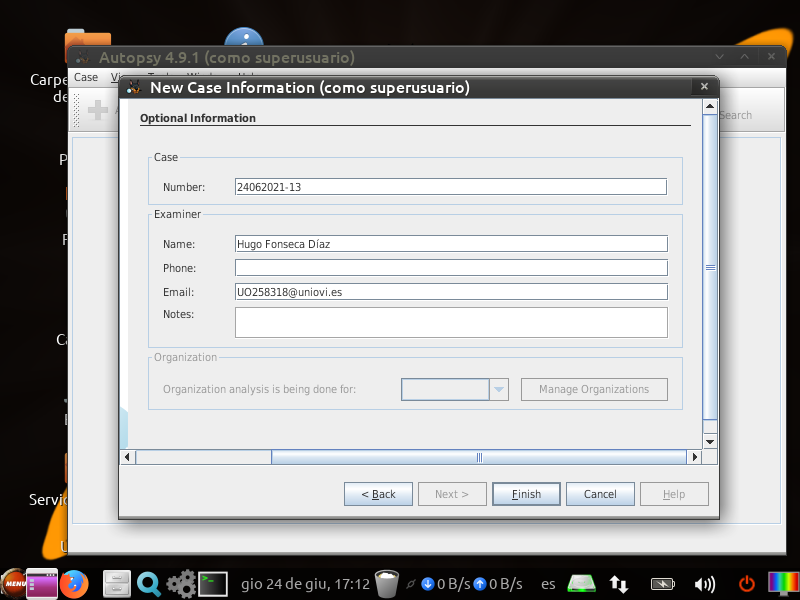
\includegraphics[scale=0.7]{p03/e13-2.png}
\end{figure}

Añadimos la imagen a analizar.

\begin{figure}[H]
    \caption{Ejercicio 13: Selección de la imagen}
    \centering
    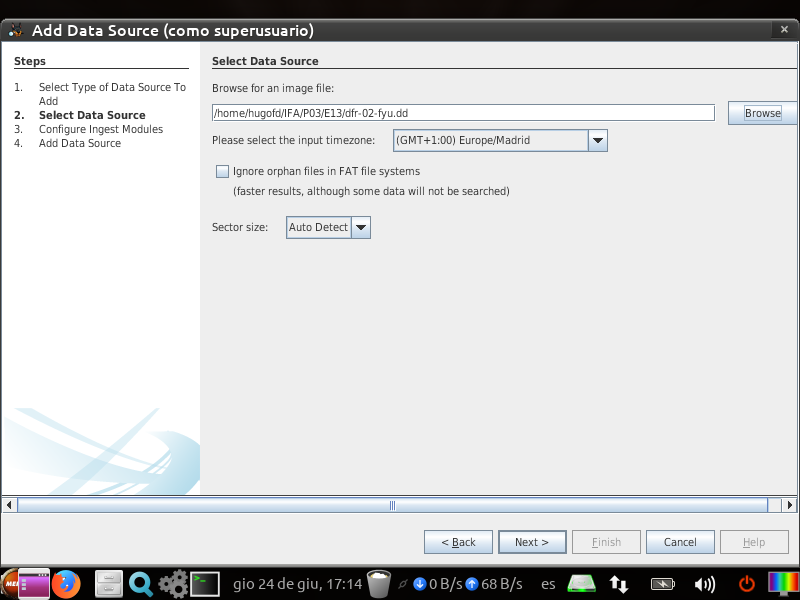
\includegraphics[scale=0.7]{p03/e13-3.png}
\end{figure}

Se seleccionan los módulos de identificación de tipos de fichero y \textit{PhotoRec Carver}.

\begin{figure}[H]
    \caption{Ejercicio 13: Selección de módulos}
    \centering
    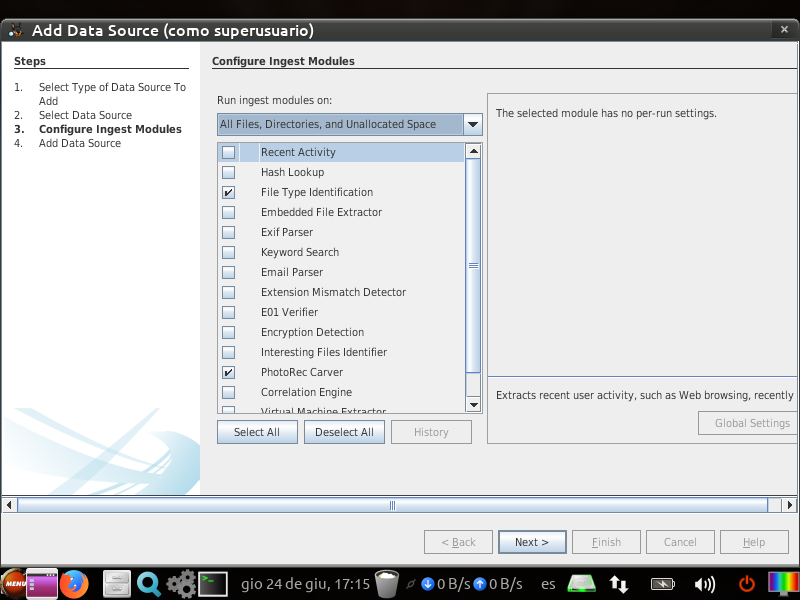
\includegraphics[scale=0.7]{p03/e13-4.png}
\end{figure}

Se obtienen los resultados del análisis con los que se responderán a las diferentes cuestiones del ejercicio.

\begin{figure}[H]
    \caption{Ejercicio 13: Resultados del análisis}
    \centering
    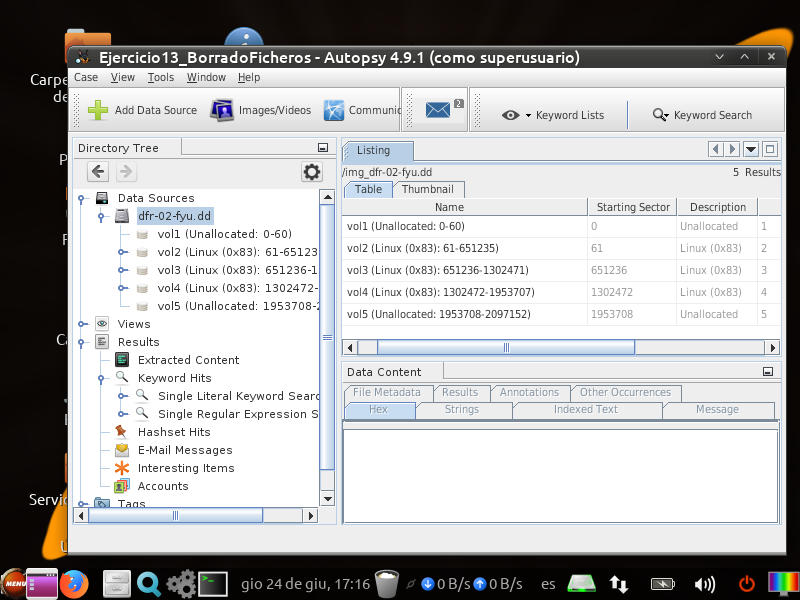
\includegraphics[scale=0.7]{p03/e13-5.png}
\end{figure}

a)

\begin{table}[H]
    \centering
    \begin{tabular}{|c|c|c|c|}
        \hline
        Número partición & Sector comienzo & Sector finalización & Tipo Sistema de Ficheros \\
        \hline\hline
        1 & 0 & 60 & Unallocated \\
        \hline
        2 & 61 & 651235 & Linux \\
        \hline
        3 & 651236 & 1302471 & Linux \\
        \hline
        4 & 1302472 & 1953707 & Linux \\
        \hline
        5 & 1953708 & 2097152 & Unallocated \\
        \hline
    \end{tabular}
\end{table}

b) Para responder a esta cuestión se observan los resultados de la pestaña 'Views'.

\begin{figure}[H]
    \caption{Ejercicio 13: Ficheros de texto plano}
    \centering
    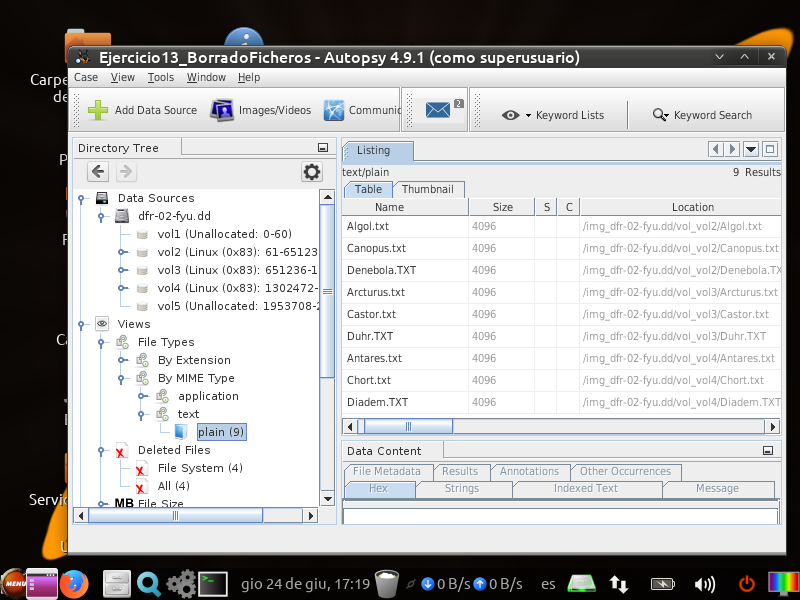
\includegraphics[scale=0.7]{p03/e13-6.png}
\end{figure}

Se puede ver que hay 9 ficheros de texto plano. Hay 4 ficheros adicionales borrados, uno llamado OrphanFiles, el cual es autogenerado por Autopsy, y tres ficheros con extensión txt pero cuyos tipos MIME no son texto plano.

c) Para rellenar esta tabla se miran los metadatos que muestra Autopsy de cada archivo borrado.

\begin{figure}[H]
    \caption{Ejercicio 13: Metadatos de los ficheros borrados}
    \centering
    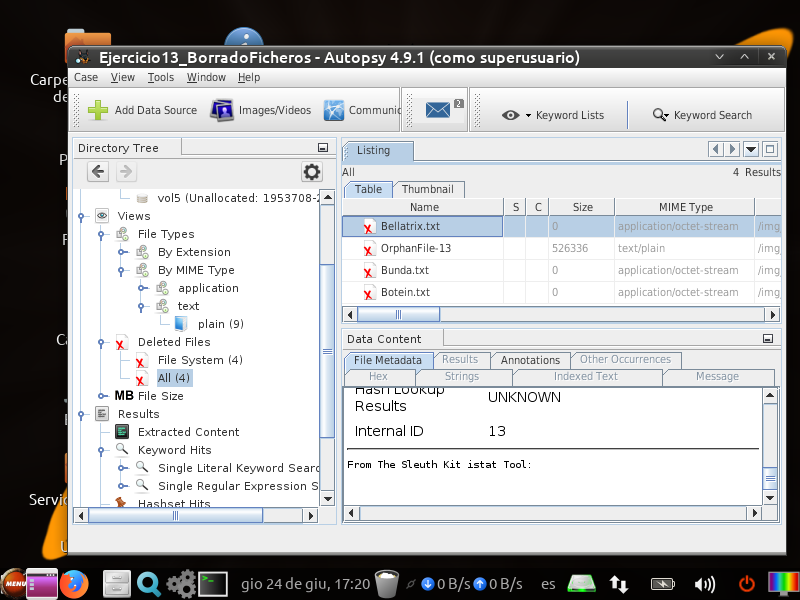
\includegraphics[scale=0.7]{p03/e13-7.png}
\end{figure}

Como se puede observar hay menos metadatos sobre los ficheros borrados que en el ejercicio anterior, por lo que habrá secciones de la tabla sin rellenar.

\begin{table}[H]
    \centering
    \begin{tabular}{|c|c|c|c|p{2cm}|p{2cm}|p{2cm}|}
        \hline
        Nombre & Tamaño & Partición & Sector relativo & Acceso (GMT) & Modificación (GMT) & Creación (GMT) \\
        \hline\hline
        Bellatrix.txt & 0 & vol 2 & - & - & - & - \\
        \hline
        Bunda.txt & 0 & vol 3 & - & 1999/01/02 08:04:00 & 2011/10/16 18:52:31 & 2011/10/16 18:52:31 \\
        \hline
        Botein.txt & 0 & vol 4 & - & 1999/01/02 08:05:00 & 2011/10/16 18:52:31 & 2011/10/16 18:52:31 \\
        \hline
    \end{tabular}
\end{table}

d) Se muestran a continuación las líneas de tiempo de los tres ficheros borrados, en el filtro de la parte izquierda de la captura se observa el fichero actual.

\begin{figure}[H]
    \caption{Ejercicio 13: Línea temporal de \textit{Bellatrix.txt}}
    \centering
    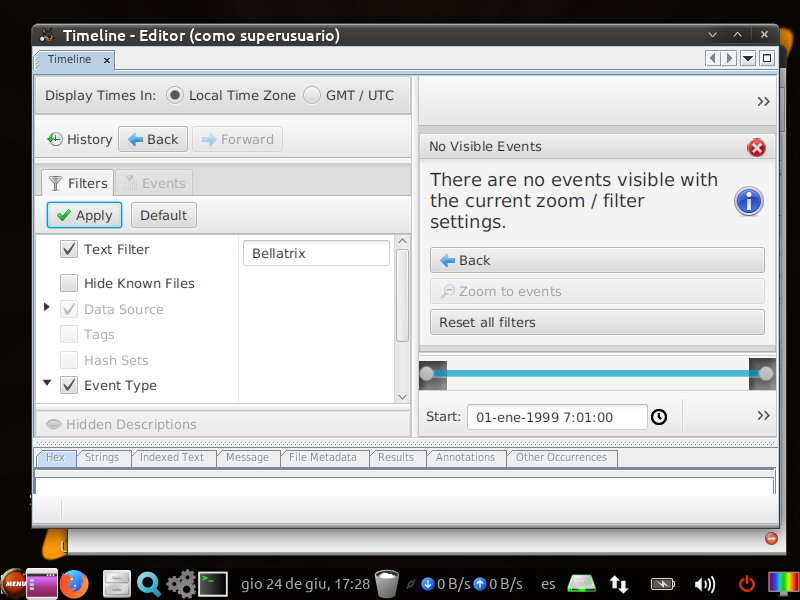
\includegraphics[scale=0.7]{p03/e13-8.png}
\end{figure}

Se observa que no hay datos para \textit{Bellatrix.txt}

\begin{figure}[H]
    \caption{Ejercicio 13: Línea temporal de \textit{Bunda.txt}}
    \centering
    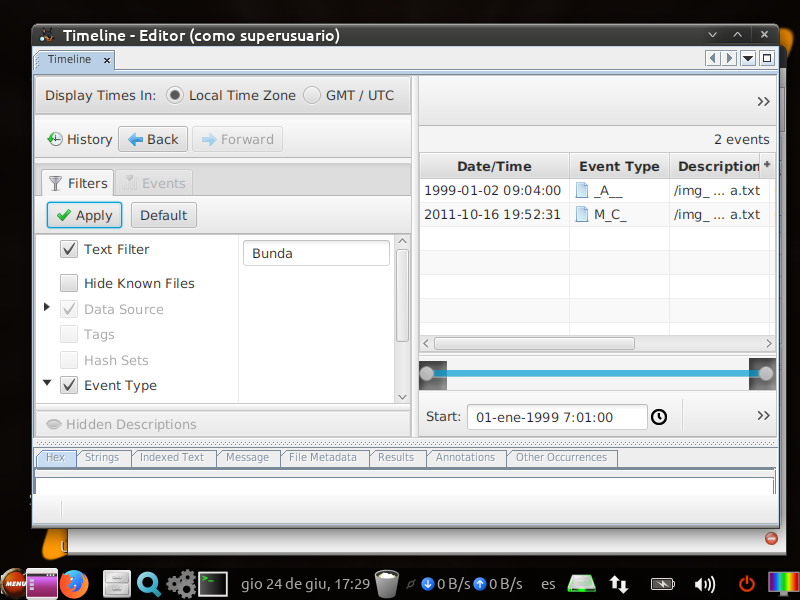
\includegraphics[scale=0.7]{p03/e13-9.png}
\end{figure}

\begin{figure}[H]
    \caption{Ejercicio 13: Línea temporal de \textit{Botein.txt}}
    \centering
    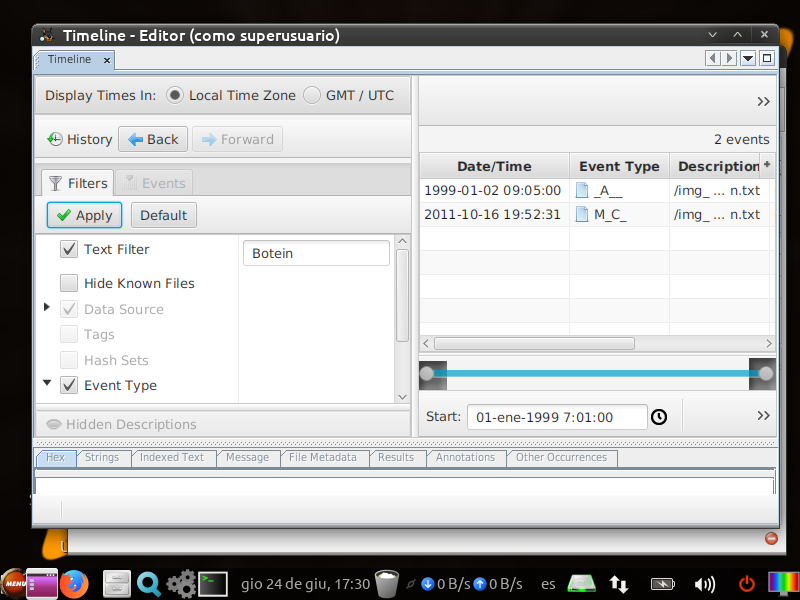
\includegraphics[scale=0.7]{p03/e13-10.png}
\end{figure}

Para \textit{Bunda.txt} y \textit{Botein.txt} sí que se recuperan datos.

\subsection{Ejercicio 14}

\begin{figure}[H]
    \caption{Ejercicio 14: Enunciado (I).}
  \centering
  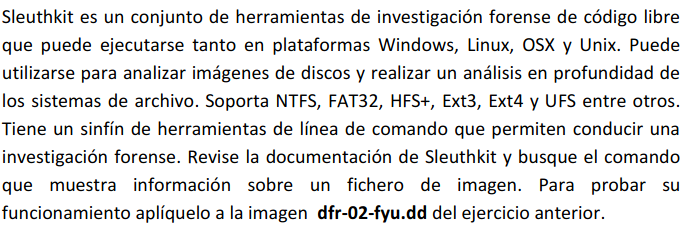
\includegraphics[scale=0.7]{other/enunciado_p03_e14-1.png}
\end{figure}

\begin{figure}[H]
    \caption{Ejercicio 14: Enunciado (II).}
  \centering
  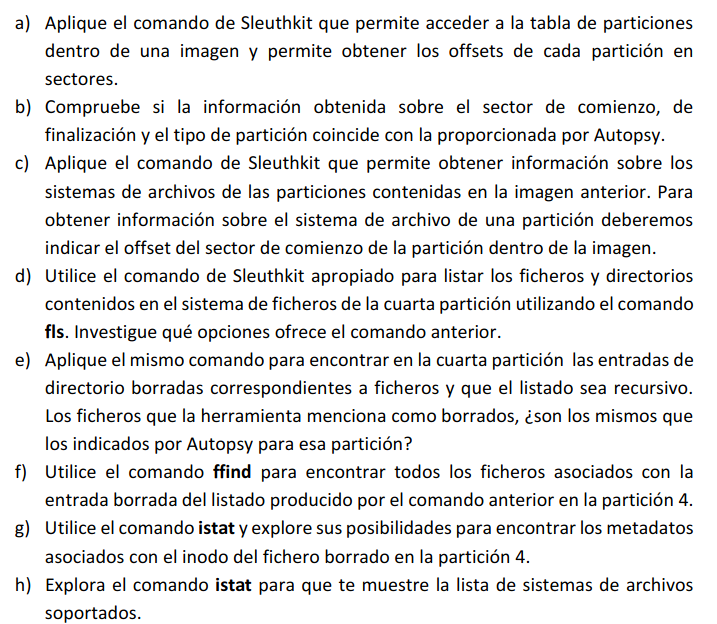
\includegraphics[scale=0.7]{other/enunciado_p03_e14-2.png}
\end{figure}

Se responde a continuación a las diferentes cuestiones planteadas por el ejercicio.

a) Se utiliza el comando \verb|mmls|, que lista las particiones con sus sectores de inicio y fin, entre otros datos.

\begin{figure}[H]
    \caption{Ejercicio 14: Salida del comando \textit{mmls}}
    \centering
    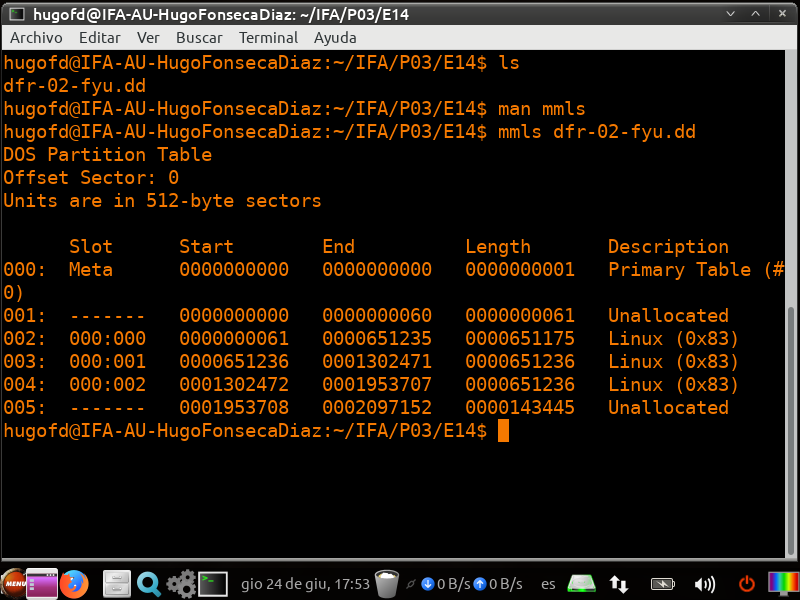
\includegraphics[scale=0.7]{p03/e14-1.png}
\end{figure}

b) Sí, la información es consistente entre ambas herramientas.

c) Se usa el comando \verb|fsstat|, con la flag \textit{t} para mostrar solo el tipo de partición y la flag \textit{o} para pasarle al comando el sector donde comienza la partición.

\begin{figure}[H]
    \caption{Ejercicio 14: Salida del comando \textit{fsstat} para las diferentes particiones}
    \centering
    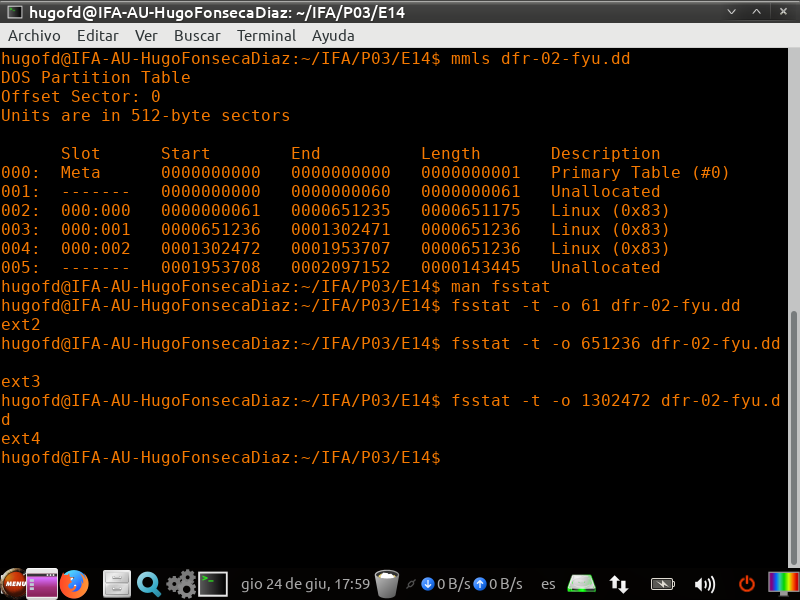
\includegraphics[scale=0.7]{p03/e14-2.png}
\end{figure}

d) Se utiliza el comando \verb|fls| que recibe como argumentos, entre otros, el comienzo del sector de la partición que se quiere analizar.

\begin{figure}[H]
    \caption{Ejercicio 14: Salida del comando \textit{fls} con las flags \textit{ro}}
    \centering
    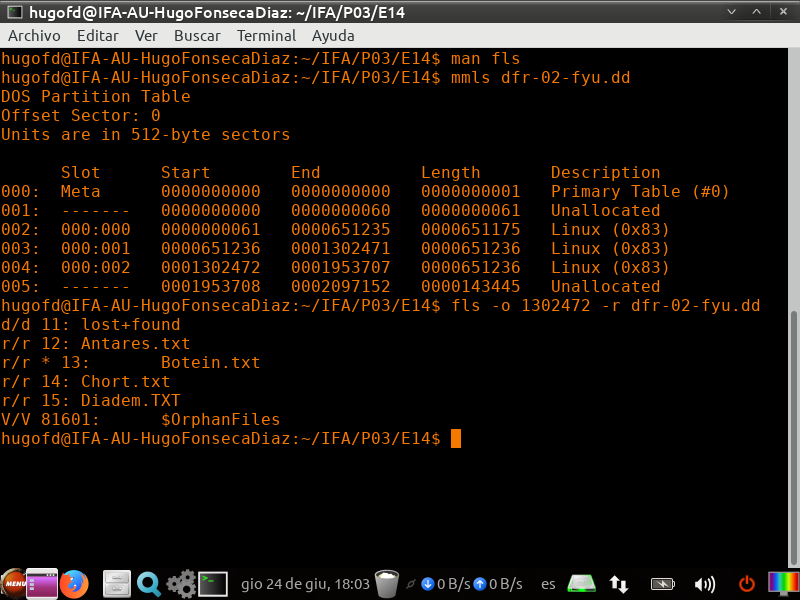
\includegraphics[scale=0.7]{p03/e14-3.png}
\end{figure}

e) Se usa ahora el comando \verb|fls| con las flags \textit{dFro}, \textit{d} muestra solo elementos borrados, \textit{F} muestra solo ficheros, \textit{r} es para que la búsqueda sea recursiva y \textit{o} para introducir el comienzo del sector de la partición.

\begin{figure}[H]
    \caption{Ejercicio 14: Salida del comando \textit{fls} con las flags \textit{dFro}}
    \centering
    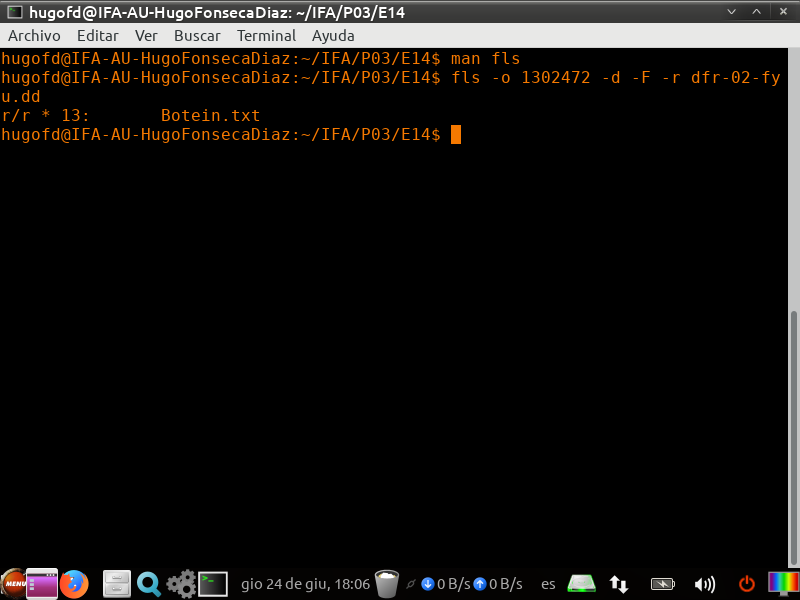
\includegraphics[scale=0.7]{p03/e14-4.png}
\end{figure}

f) Se utiliza el comando \verb|ffind| con las flags \textit{oa}, \textit{o} para introducir el comienzo del sector de la partición y \textit{a} para buscar todos los ficheros asociados. Se le pasa al comando el inodo del elemento que se está buscando, en este caso el 13.

\begin{figure}[H]
    \caption{Ejercicio 14: Salida del comando \textit{ffind}}
    \centering
    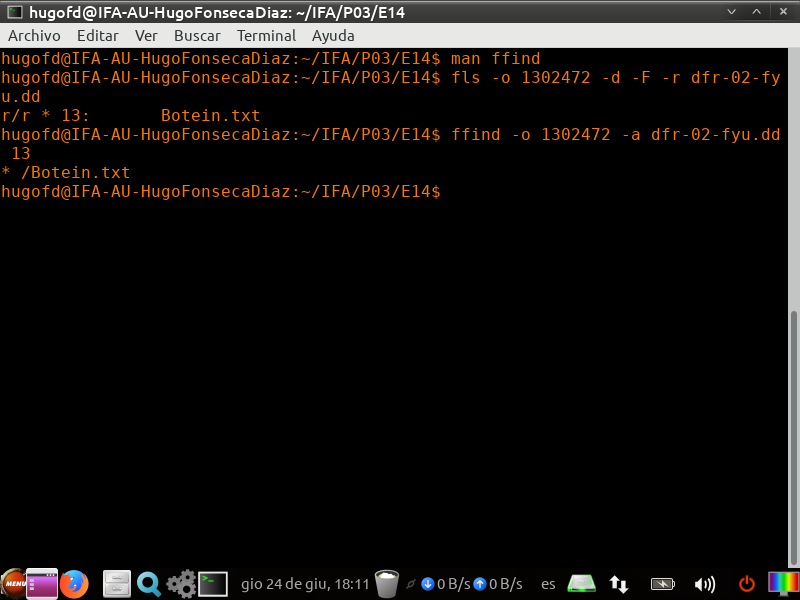
\includegraphics[scale=0.7]{p03/e14-5.png}
\end{figure}

g) Se usa el comando \verb|istat| pasandole como argumento el comienzo del sector de la partición y el inodo a buscar.

\begin{figure}[H]
    \caption{Ejercicio 14: Salida del comando \textit{istat} para el inodo 13}
    \centering
    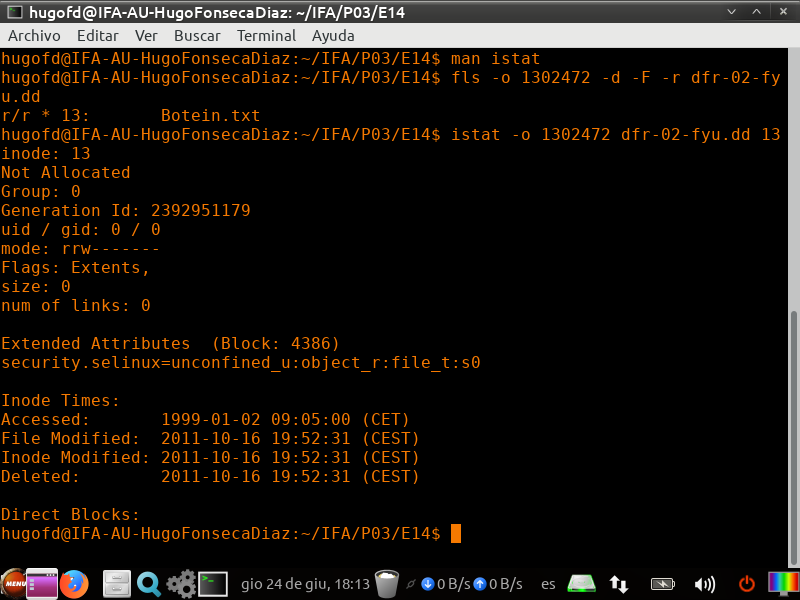
\includegraphics[scale=0.7]{p03/e14-6.png}
\end{figure}

h) Se usa el comando \verb|istat| con la flag \textit{f} y el argumento \textit{list}.

\begin{figure}[H]
    \caption{Ejercicio 14: Salida del comando \textit{istat -f list}}
    \centering
    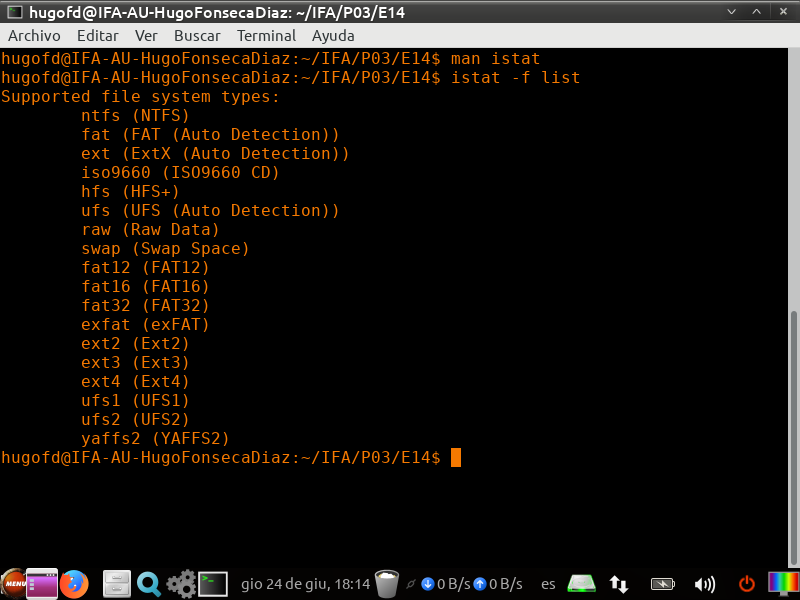
\includegraphics[scale=0.7]{p03/e14-7.png}
\end{figure}

\subsection{Ejercicio 19}

\begin{figure}[H]
    \caption{Ejercicio 19: Enunciado.}
  \centering
  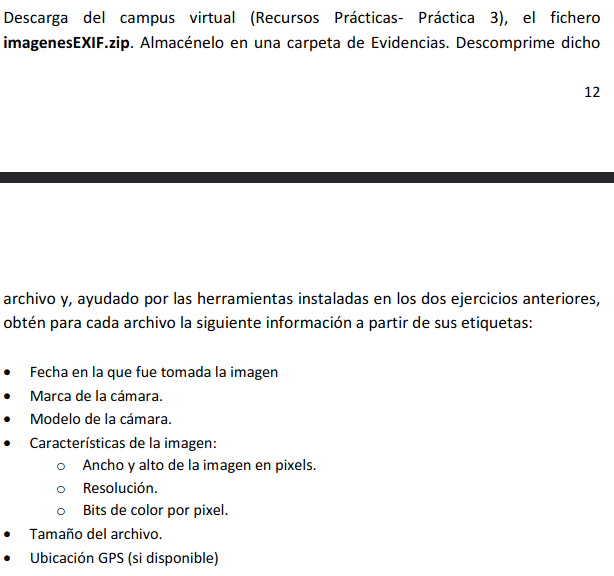
\includegraphics[scale=0.7]{other/enunciado_p03_e19.png}
\end{figure}

Para este ejercicio se pueden realizar dos aproximaciones, una es mediante la interfaz gráfica de \verb|exiftool| para el sistema operativo Windows y la otra mediante el propio comando de consola \verb|exiftool|. Se probarán las dos para la primera imagen y se realizará el resto de imagenes con el comando de consola.

\subsubsection{Imagen 1}

\begin{figure}[H]
    \caption{Ejercicio 19: Metadatos de la imagen 1 con la interfaz gráfica de \textit{exiftool} (I)}
    \centering
    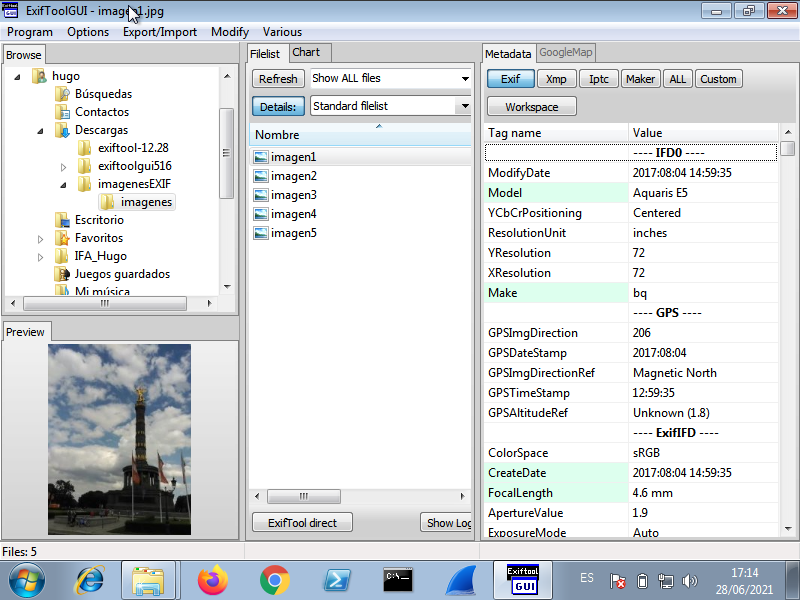
\includegraphics[scale=0.7]{p03/e19-1.png}
\end{figure}

\begin{figure}[H]
    \caption{Ejercicio 19: Metadatos de la imagen 1 con la interfaz gráfica de \textit{exiftool} (II)}
    \centering
    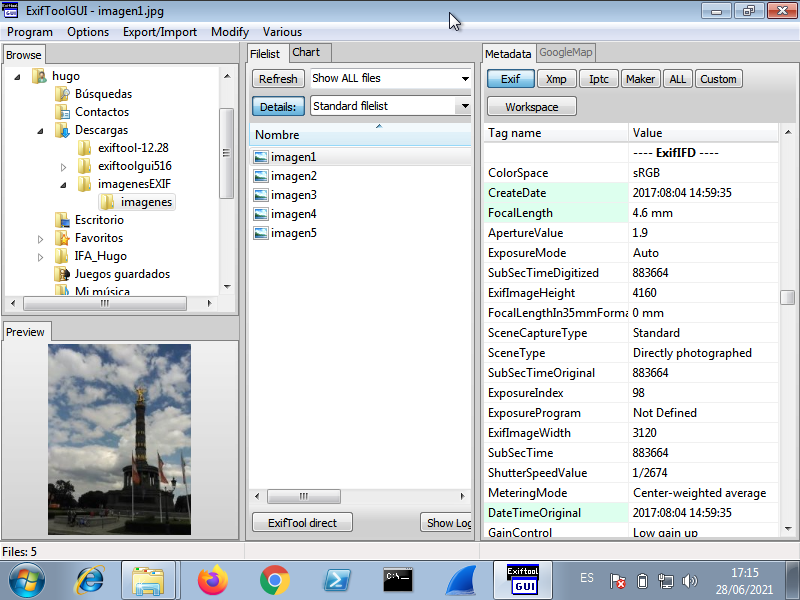
\includegraphics[scale=0.7]{p03/e19-2.png}
\end{figure}

\begin{figure}[H]
    \caption{Ejercicio 19: Metadatos de la imagen 1 con el comando \textit{exiftool} (I)}
    \centering
    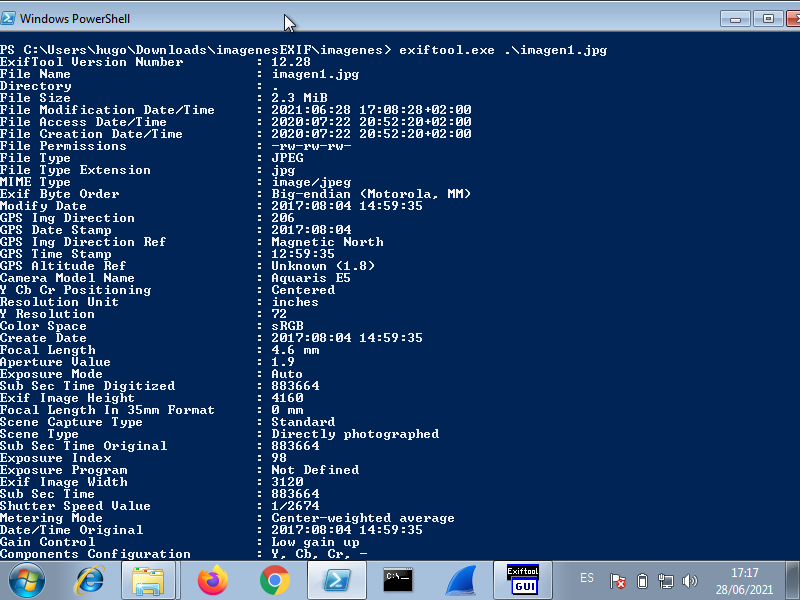
\includegraphics[scale=0.7]{p03/e19-3.png}
\end{figure}

\begin{figure}[H]
    \caption{Ejercicio 19: Metadatos de la imagen 1 con el comando \textit{exiftool} (II)}
    \centering
    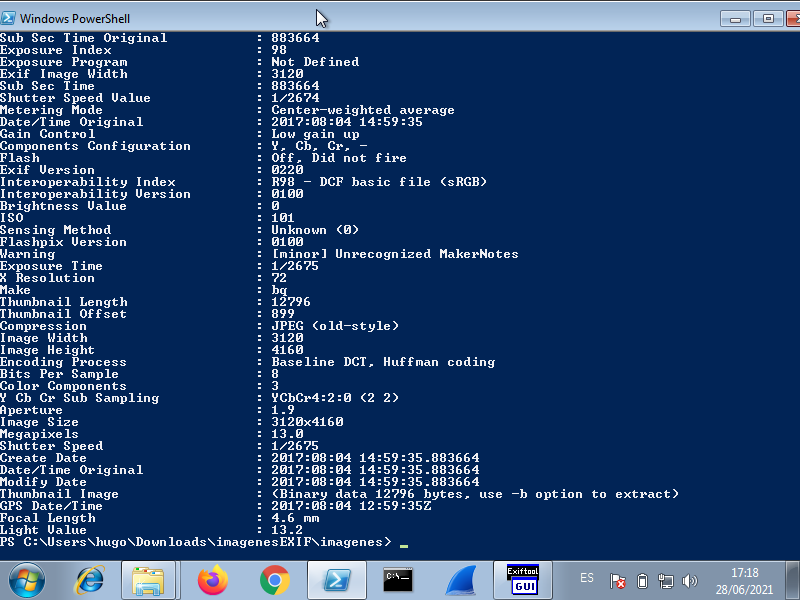
\includegraphics[scale=0.7]{p03/e19-4.png}
\end{figure}

Con lo anterior visto, se procede a rellenar la lista de datos requeridos:

\begin{itemize}
    \item \textbf{Fecha en la que fue tomada la imagen}: 2017/08/04 14:59:35 
    \item \textbf{Marca de la cámara}: bq
    \item \textbf{Modelo de la cámara}: Aquaris E5
    \item \textbf{Características de la imagen}:
        \begin{itemize}
            \item \textbf{Ancho y alto en píxeles}: Ancho 3120, alto 4160
            \item \textbf{Resolución}: 3120x4160
            \item \textbf{Bits de color por pixel}: 8 bits y 3 canales, así que 24 bits de color por pixel
        \end{itemize}
    \item \textbf{Tamaño del archivo}: 2.3MiB
    \item \textbf{Ubicación GPS}: No está presente
\end{itemize}


\subsubsection{Imagen 2}

\begin{figure}[H]
    \caption{Ejercicio 19: Metadatos de la imagen 2 con el comando \textit{exiftool} (I)}
    \centering
    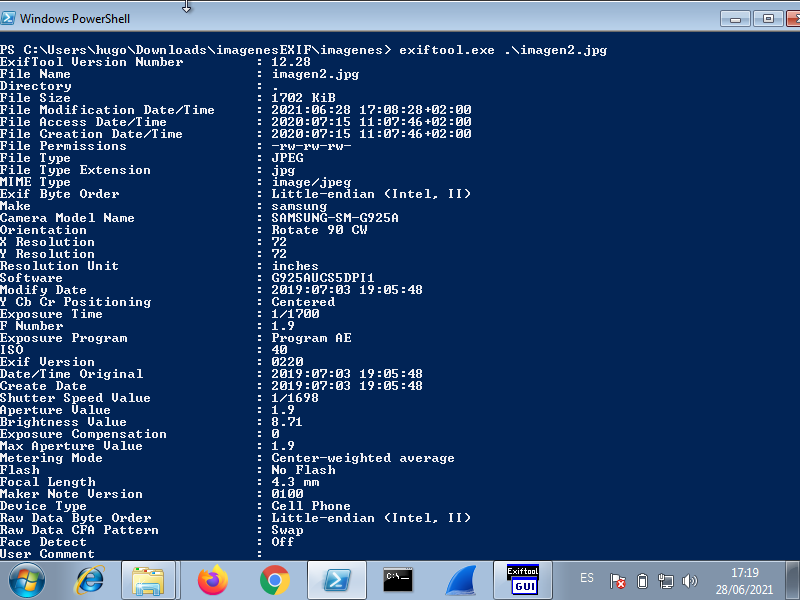
\includegraphics[scale=0.7]{p03/e19-5.png}
\end{figure}

\begin{figure}[H]
    \caption{Ejercicio 19: Metadatos de la imagen 2 con el comando \textit{exiftool} (II)}
    \centering
    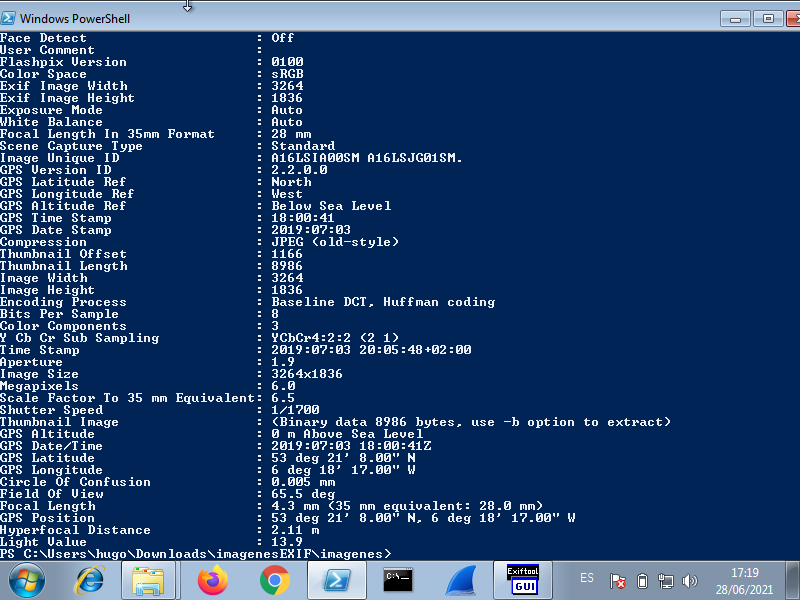
\includegraphics[scale=0.7]{p03/e19-6.png}
\end{figure}

Con lo anterior visto, se procede a rellenar la lista de datos requeridos:

\begin{itemize}
    \item \textbf{Fecha en la que fue tomada la imagen}: 2019/07/03 19:05:48 
    \item \textbf{Marca de la cámara}: Samsung
    \item \textbf{Modelo de la cámara}: SAMSUNG-SM-G925A
    \item \textbf{Características de la imagen}:
        \begin{itemize}
            \item \textbf{Ancho y alto en píxeles}: Ancho 3264, alto 1836
            \item \textbf{Resolución}: 3264x1836
            \item \textbf{Bits de color por pixel}: 8 bits y 3 canales, así que 24 bits de color por pixel
        \end{itemize}
    \item \textbf{Tamaño del archivo}: 1702 KiB
    \item \textbf{Ubicación GPS}: Latitud 53 deg 21' 8.00" North, longitud 6 deg 18' 17.00" West
\end{itemize}

\subsubsection{Imagen 3}

\begin{figure}[H]
    \caption{Ejercicio 19: Metadatos de la imagen 3 con el comando \textit{exiftool} (I)}
    \centering
    \includegraphics[scale=0.7]{p03/e19-7.png}
\end{figure}

\begin{figure}[H]
    \caption{Ejercicio 19: Metadatos de la imagen 3 con el comando \textit{exiftool} (II)}
    \centering
    \includegraphics[scale=0.7]{p03/e19-8.png}
\end{figure}

Con lo anterior visto, se procede a rellenar la lista de datos requeridos:

\begin{itemize}
    \item \textbf{Fecha en la que fue tomada la imagen}: 2019/06/16 13:57:37
    \item \textbf{Marca de la cámara}: Samsung
    \item \textbf{Modelo de la cámara}: SAMSUNG-SM-G925A
    \item \textbf{Características de la imagen}:
        \begin{itemize}
            \item \textbf{Ancho y alto en píxeles}: Ancho 3264, alto 1836
            \item \textbf{Resolución}: 3264x1836
            \item \textbf{Bits de color por pixel}: 8 bits y 3 canales, así que 24 bits de color por pixel
        \end{itemize}
    \item \textbf{Tamaño del archivo}: 1806 KiB
    \item \textbf{Ubicación GPS}: Latitud 38 deg 42' 51.00" North, longitud 9 deg 8' 23.00" West
\end{itemize}

\subsubsection{Imagen 4}

\begin{figure}[H]
    \caption{Ejercicio 19: Metadatos de la imagen 4 con el comando \textit{exiftool} (I)}
    \centering
    \includegraphics[scale=0.7]{p03/e19-9.png}
\end{figure}

\begin{figure}[H]
    \caption{Ejercicio 19: Metadatos de la imagen 4 con el comando \textit{exiftool} (II)}
    \centering
    \includegraphics[scale=0.7]{p03/e19-10.png}
\end{figure}

Con lo anterior visto, se procede a rellenar la lista de datos requeridos:

\begin{itemize}
    \item \textbf{Fecha en la que fue tomada la imagen}: 2017/08/09 11:58:23 
    \item \textbf{Marca de la cámara}: bq
    \item \textbf{Modelo de la cámara}: Aquaris E5
    \item \textbf{Características de la imagen}:
        \begin{itemize}
            \item \textbf{Ancho y alto en píxeles}: Ancho 4160, alto 3120
            \item \textbf{Resolución}: 4160x3120
            \item \textbf{Bits de color por pixel}: 8 bits y 3 canales, así que 24 bits de color por pixel
        \end{itemize}
    \item \textbf{Tamaño del archivo}: 3.5 MiB
    \item \textbf{Ubicación GPS}: No está presente 
\end{itemize}

\subsubsection{Imagen 5}

\begin{figure}[H]
    \caption{Ejercicio 19: Metadatos de la imagen 5 con el comando \textit{exiftool} (I)}
    \centering
    \includegraphics[scale=0.7]{p03/e19-11.png}
\end{figure}

\begin{figure}[H]
    \caption{Ejercicio 19: Metadatos de la imagen 5 con el comando \textit{exiftool} (II)}
    \centering
    \includegraphics[scale=0.7]{p03/e19-12.png}
\end{figure}

Con lo anterior visto, se procede a rellenar la lista de datos requeridos:

\begin{itemize}
    \item \textbf{Fecha en la que fue tomada la imagen}: 2014/09/07 13:10:28 
    \item \textbf{Marca de la cámara}: No está presente
    \item \textbf{Modelo de la cámara}: No está presente
    \item \textbf{Características de la imagen}:
        \begin{itemize}
            \item \textbf{Ancho y alto en píxeles}: Ancho 2448, alto 3264
            \item \textbf{Resolución}: 2448x3264
            \item \textbf{Bits de color por pixel}: 8 bits y 3 canales, así que 24 bits de color por pixel
        \end{itemize}
    \item \textbf{Tamaño del archivo}: 1118 KiB
    \item \textbf{Ubicación GPS}: No está presente
\end{itemize}



% Práctica 04
\section{Práctica 04}

\subsection{Ejercicio 7}

\begin{figure}[H]
    \caption{Ejercicio 7: Enunciado (I).}
  \centering
  \includegraphics[scale=0.7]{other/enunciado_p04_e7-1.png}
\end{figure}

\begin{figure}[H]
    \caption{Ejercicio 7: Enunciado (II).}
  \centering
  \includegraphics[scale=0.7]{other/enunciado_p04_e7-2.png}
\end{figure}

\begin{figure}[H]
    \caption{Ejercicio 7: Enunciado (III).}
  \centering
  \includegraphics[scale=0.7]{other/enunciado_p04_e7-3.png}
\end{figure}

Debido a que la máquina que se utiliza para hacer los ejercicios tiene un sistema operativo Linux, el ejercicio 7 se realizó en el ordenador de un familiar. Se han incluído datos personales en las capturas para asegurar la autoría de las mismas.

Lo primero que se debe hacer en este ejercicio es crear un caso en la herramienta \textit{Belkasoft Evidence Center X}.

\begin{figure}[H]
    \caption{Ejercicio 4: Creación del caso}
    \centering
    \includegraphics[scale=0.6]{p04/e7-1.PNG}
\end{figure}

Se selecciona la imagen.

\begin{figure}[H]
    \caption{Ejercicio 4: Selección de la imagen}
    \centering
    \includegraphics[scale=0.7]{p04/e7-2.PNG}
\end{figure}

Se eligen las opciones que pide el enunciado.

\begin{figure}[H]
    \caption{Ejercicio 4: Tipo de análisis}
    \centering
    \includegraphics[scale=0.7]{p04/e7-3.PNG}
\end{figure}

Se configuran las opciones de análisis avanzadas.

\begin{figure}[H]
    \caption{Ejercicio 4: Opciones de análisis avanzadas}
    \centering
    \includegraphics[scale=0.4]{p04/e7-4.PNG}
\end{figure}

Se ejecuta el análisis, nótese que el tiempo de ejecución es bastante superior al que se obtuvo al analizar la misma imagen con Autopsy, aunque los resultados son más completos.

\begin{figure}[H]
    \caption{Ejercicio 4: Ejecución del análisis}
    \centering
    \includegraphics[scale=0.4]{p04/e7-6.PNG}
\end{figure}

Finalizado el análisis, se comienza a responder a las preguntas del ejercicio. Cabe mencionar que el análisis ha finalizado con errores, pero considerando los resultados obtenidos y viendo el tiempo de ejecución, no se cree conveniente reintentar el análisis.

\begin{figure}[H]
    \caption{Ejercicio 4: Resultado del análisis}
    \centering
    \includegraphics[scale=0.4]{p04/e7-9.PNG}
\end{figure}

rr) Como se puede observar en la anterior captura, hay 195 documentos identificados.

ss) 

\begin{figure}[H]
    \caption{Ejercicio 4: Documentos de tipo \textit{pdf}}
    \centering
    \includegraphics[scale=0.4]{p04/e7-10.PNG}
\end{figure}

Hay un solo documento de tipo \textit{pdf}, llamado \textit{forensics.pdf}.

tt)

\begin{figure}[H]
    \caption{Ejercicio 4: URLs visitadas}
    \centering
    \includegraphics[scale=0.4]{p04/e7-11.PNG}
\end{figure}

No hay ninguna url correspondiente a \textit{Facebook}.

uu)

\begin{figure}[H]
    \caption{Ejercicio 4: Cookies relativas a \textit{Facebook}}
    \centering
    \includegraphics[scale=0.4]{p04/e7-12.PNG}
\end{figure}

Aunque no haya ninguna url visitada correspondiente a \textit{Facebook}, inspeccionando las cookies se puede observar que la hora de la última visita a \textit{Facebook} fue a las 13:42:23 del día 2019/11/09.

vv)

\begin{figure}[H]
    \caption{Ejercicio 4: Imágenes identificadas}
    \centering
    \includegraphics[scale=0.4]{p04/e7-13.PNG}
\end{figure}

Como se observa en la figura, se identificaron algo más de 30.000 imágenes.

ww)

\begin{figure}[H]
    \caption{Ejercicio 4: Imágenes en formato \textit{jpg}}
    \centering
    \includegraphics[scale=0.4]{p04/e7-14.PNG}
\end{figure}

Se han encontrado 1011 imágenes en formato \textit{jpg}. Sin embargo, se han buscado mediante el nombre de usuario, lo que no es la mejor aproximación (ya que podría haber imágenes con tipo MIME \textit{jpg} que no tuvieran extensión), pero como no se encontró ningún filtro por tipo MIME se deja esta solución. Sería una funcionalidad interesante para el programa (a menos que ya exista, en cuyo caso no pudo encontrarse).

xx)

\begin{figure}[H]
    \caption{Ejercicio 4: Reconocimiento de rostros}
    \centering
    \includegraphics[scale=0.4]{p04/e7-15.PNG}
\end{figure}

Hay 100 imágenes con rostros detectados, aunque en su mayoría se trata de \textit{emojis}, y muchos de ellos ni siquiera son rostros.

yy)

\begin{figure}[H]
    \caption{Ejercicio 4: Eventos de calendario}
    \centering
    \includegraphics[scale=0.4]{p04/e7-16.PNG}
\end{figure}

Se han identificado 54 eventos de calendario.

zz)

\begin{figure}[H]
    \caption{Ejercicio 4: Eventos en Los Ángeles}
    \centering
    \includegraphics[scale=0.4]{p04/e7-17.PNG}
\end{figure}

Solo uno se desarrolla en Los Ángeles.

aaa) La fecha de comienzo del evento puede verse en la anterior captura, es el 2016/04/23 a las 8:00:00.



% Práctica 05
\section{Práctica 05}

\subsection{Ejercicio 5}

\begin{figure}[H]
    \caption{Ejercicio 5: Enunciado.}
  \centering
  \includegraphics[scale=0.7]{other/enunciado_p05_e5.png}
\end{figure}

Se realiza una conexión al campus virtual con el navegador Firefox en navegación privada.

\begin{figure}[H]
  \caption{Ejercicio 5: Campus virtual}
  \centering
    \includegraphics[scale=0.7]{p05/e5-1.png}
\end{figure}

Se utiliza la aplicación de Nirsoft llamada \textit{CurrPorts}.

\begin{figure}[H]
    \caption{Ejercicio 5: \textit{CurrPorts}}
  \centering
    \includegraphics[scale=0.7]{p05/e5-2.png}
\end{figure}

Se ordena la salida de la aplicación por nombre de proceso para poder visualizar todos los procesos de Firefox.

\begin{figure}[H]
    \caption{Ejercicio 5: \textit{CurrPorts} - Firefox}
  \centering
    \includegraphics[scale=0.7]{p05/e5-3.png}
\end{figure}

Curiosamente, no sale ninguna conexión con el campus virtual. Se prueba ahora con una ventana de navegación privada del navegador Chrome.

\begin{figure}[H]
    \caption{Ejercicio 5: \textit{CurrPorts} - Chrome (I)}
  \centering
    \includegraphics[scale=0.7]{p05/e5-4.png}
\end{figure}

\begin{figure}[H]
    \caption{Ejercicio 5: \textit{CurrPorts} - Chrome (II)}
  \centering
    \includegraphics[scale=0.7]{p05/e5-5.png}
\end{figure}

Ahora sí que se visualizan las conexiones con la intranet de uniovi. Se ha podido comprobar por casualidad que Firefox ofrece menos información sobre sus conexiones que Chrome, quizás por su mayor enfoque en la privacidad de los usuarios. Se desconoce si esto solo ocurre al usar navegación privada.

Si se quisiera obtener esta información por consola, lo primero habría que tener cuidado porque los comandos del equipo intervenido pueden no dar información confiable, pero suponiendo que es una operación segura, se deberá usar el comando \verb|netstat|. Se listan a continuación sus opciones.

\begin{figure}[H]
    \caption{Ejercicio 5: \textit{netstat -h}}
  \centering
    \includegraphics[scale=0.7]{p05/e5-6.png}
\end{figure}

Lo que pide el ejercicio puede obtenerse mediante las flags \textit{bfp}, cuyas funcionalidades fueron listadas en la anterior captura. La opción \textit{p} requiere como argumento el nombre del protocolo que se está buscando, siendo en este caso TCP.

\begin{figure}[H]
    \caption{Ejercicio 5: \textit{netstat -b -f -p TCP}}
  \centering
    \includegraphics[scale=0.7]{p05/e5-7.png}
\end{figure}

La operación debe realizarse con permisos de administrador.

\subsection{Ejercicio 25}

\begin{figure}[H]
    \caption{Ejercicio 25: Enunciado.}
  \centering
  \includegraphics[scale=0.7]{other/enunciado_p05_e25.png}
\end{figure}

Este ejercicio, como el 7 de la práctica 4, fue realizado en el ordenador de un familiar, ya que Virtualbox en Linux no parece reconocer los USBs conectados a la máquina anfitriona, lo que impide realizar los filtros.

Lo primero que se va a hacer es formatear un USB con el sistema de archivos NTFS y posteriormente se van a crear dos particiones, una en NTFS y otra en FAT32.

\begin{figure}[H]
    \caption{Ejercicio 25: USB con las particiones}
  \centering
    \includegraphics[scale=0.4]{p05/e25-1.PNG}
\end{figure}

Ahora, se introducen ficheros de ejemplo en ambas particiones y posteriormente se borran dichas particiones.

\begin{figure}[H]
    \caption{Ejercicio 25: Borrado de las particiones}
  \centering
    \includegraphics[scale=0.4]{p05/e25-2.PNG}
\end{figure}

Se añade el filtro del usb y se conecta a la máquina virtual. Aquí se produce un problema inesperado, tanto la máquina anfitriona con Linux como la del familiar con Windows son el mismo modelo, y ambas cuentan solo con puertos USB 3.0. Como Windows 7 no tiene soporte para USB 3.0 se intentaron instalar los drivers necesarios, pero la operación no pudo ejecutarse.

\begin{figure}[H]
    \caption{Ejercicio 25: Fallo al instalar los drivers de los puertos de USB 3.0}
  \centering
    \includegraphics[scale=0.8]{p05/e25-3.png}
\end{figure}

\begin{figure}[H]
    \caption{Ejercicio 25: Filtro USB configurado correctamente}
  \centering
    \includegraphics[scale=0.4]{p05/e25-5.PNG}
\end{figure}

Como no se puede conectar el USB al equipo virtual, se seguirá el ejercicio hasta donde sea posible. La aplicación que se usaría para resolver el ejercicio se encuentra en la carpeta \textit{PhotoRec}, y se llama \textit{testdisk}.

\begin{figure}[H]
    \caption{Ejercicio 25: Aplicación \textit{testdisk}}
  \centering
    \includegraphics[scale=0.8]{p05/e25-6.png}
\end{figure}

Aquí se debería seleccionar el USB correcto, elegir el tipo de la tabla de particiones, y realizar un análisis. Lamentablemente, debido a los problemas antes mencionados, no se ha podido continuar con el ejercicio.

\subsection{Ejercicio 31}

\begin{figure}[H]
    \caption{Ejercicio 31: Enunciado.}
  \centering
  \includegraphics[scale=0.7]{other/enunciado_p05_e31.png}
\end{figure}

Se localiza el hilo de \textit{Twitter} mencionado en el enunciado.

\begin{figure}[H]
    \caption{Ejercicio 31: Hilo de Twitter}
  \centering
    \includegraphics[scale=0.8]{p05/e31-1.png}
\end{figure}

Una vez obtenida la URL de la imagen del hilo, se realiza una búsqueda inversa de la misma mediante el buscador Google con las palabras clave 'trump' y 'niños'.

\begin{figure}[H]
    \caption{Ejercicio 31: Búsqueda inversa}
  \centering
    \includegraphics[scale=0.8]{p05/e31-2.png}
\end{figure}

Se entra a la noticia de la rama en español del medio estadounidense \textit{CNN}, y se obtiene la información mostrada en la siguiente captura.

\begin{figure}[H]
    \caption{Ejercicio 25: Noticia \textit{CNN en Español}}
  \centering
    \includegraphics[scale=0.8]{p05/e31-3.png}
\end{figure}

Según esta fuente, los niños de la imagen estaban detenidos en un centro de dentención de Arizona en el año 2014. Como nunca conviene fiarse de lo que diga una única fuente, se va a investigar en mayor profundidad. Se hace una búsqueda inversa que ocupe el periódo entre el 1 de enero de 2014 y el 1 de enero de 2015, y se obtiene la siguiente información.

\begin{figure}[H]
    \caption{Ejercicio 25: Búsqueda inversa por rango de fechas}
  \centering
    \includegraphics[scale=0.8]{p05/e31-6.png}
\end{figure}

\begin{figure}[H]
    \caption{Ejercicio 25: Noticia de \textit{azcentral}}
  \centering
    \includegraphics[scale=0.8]{p05/e31-4.png}
\end{figure}

\begin{figure}[H]
    \caption{Ejercicio 25: Noticia de \textit{The Atlantic}}
  \centering
    \includegraphics[scale=0.8]{p05/e31-5.png}
\end{figure}

Como se puede observar, la foto es verdaderamente del año 2014, en el período de la administración Obama, por lo que el hilo original usaba una imagen errónea. Esto refuerza más la idea de comprobar bien las fuentes de información a las que estamos sometidos cada día para no caer en la desinformación, y para que nuestros argumentos tengan una mayor base verídica que les de más peso. 



\newpage

\section{Índice de figuras}

\listoffigures



\end{document}




